\documentclass{article}
%
\usepackage{lineno,hyperref}
\modulolinenumbers[5]
%
\usepackage{color}
\usepackage{multirow}
\usepackage{pgfplots}
\usepackage{caption}
\usepackage{float}
\usepackage{colortbl}
\usepackage{amsmath}
\usepackage{amssymb}
\usepackage{graphicx}
\usepackage[bottom]{footmisc}
\usepackage{cleveref}
\usepackage{pst-plot}
\usetikzlibrary{babel}
\usepackage{refcount}
\usepackage{mathtools}
\usepackage{afterpage}
\usepackage{subcaption}
%
\usepackage[english]{babel}
%\usepackage[utf8]{inputenc}
\usepackage[T1]{fontenc}
%
\pgfplotsset{compat=1.5}
\pgfplotsset
{
	width=0.5\textwidth,
	x tick label style={/pgf/number format/1000 sep=},
	enlarge x limits = 0.0,
	ymajorgrids=true,
	major tick style={draw=none},
	ymin = 0.0,
	every axis/.append style={
		every x tick label/.append style={font=\tiny},
		every y tick label/.append style={font=\tiny},
		every axis label/.append style={font=\small},
		height=37mm,
    	width=37mm,
		title style={at={(0.5,0.90)}, font=\normalfont},
		xticklabel style={yshift=4pt}
	}
}

\title{Generating Object Cluster Hierarchies for Benchmarking}
%
\author{\L{}ukasz P. Olech \and Micha\l{} Spytkowski \and Halina Kwasnicka \\ Department of Computational Intelligence\\ Wroclaw University of Science and Technology, \\ Wybrzeze Wyspianskiego 27, 50-370 Wroclaw, Poland\\ e-mail: \url{michal.spytkowski@pwr.edu.pl}, \\ \url{lukasz.olech@pwr.edu.pl}, \\ \url{halina.kwasnicka@pwr.edu.pl}}

\bibliographystyle{abbrv}

\usepackage{ulem} %dla przekreslania tekstow
\newcommand{\lukasz}[1]{\textcolor{blue}{#1}}
\newcommand{\michal}[1]{\textcolor{red}{#1}}

\begin{document}

\maketitle

\begin{abstract}
	Generation of Object Cluster Hierarchies is a new variant of Hierarchical Clustering that increasingly gains more interest in the field of Machine Learning. Being a novelty, the lack of tools for systematic analysis and comparison of Object Cluster Hierarchies inhibits its further development. In this paper, we propose a novel method for generating hierarchical structures of data based on Tree-Structured Stick Breaking Process that can be used for benchmarking. The article presents thorough empirical and theoretical analysis of the method revealing its characteristics. More importantly, the intuition how to operate with model parameters and a set of benchmarking datasets are provided. Conducted experiments show usefulness of the model as high flexibility in generating a wide range of differently-structured data is achieved. The developed generator together with proposed benchmarks are publicly available (\texttt{http://kio.pwr.edu.pl/?page\_id=396}).
\end{abstract}

\textbf{keywords:} Artificial Data, Benchmark Data, Benchmark Data Generator, Object Cluster Hierarchy, Tree-Structured Stick Breaking Process, Clustering Evaluation, Cluster Analysis.

\section{Introduction}
\label{sec:intro}
The enormity of digital data drives a rapid development of analysis methods, creating the opportunity to get the data insights from different perspectives. One of the key data analysis topics are \textit{regression}, \textit{classification}, and \textit{clustering}~\textbf{Kakkar2014,Dash2003109<-cos nowszego,Xu:2005:SCA:2325810.2327433<-cos nowszego}.

Clustering methods, in general, are still not satisfactory for a variety of data and specific goals~\cite{blundell2010discovering}. From the perspective of this research, the primary issue is a semantic gap that exists between how humans perceive hierarchies and Hierarchical Clustering methods. Human perception describes hierarchical data (e.g.,~\cite{ILSVRC15}) as possessing the following properties:
\begin{enumerate}
    \item the data can be present to any node in the hierarchy, not only leaves; and
    \item the data specificity should always be higher (at most equal) in a child node than in the corresponding parent node; and
    \item the data in a node should be more similar to data in parent and child nodes than to unrelated nodes located in different subtrees in the hierarchy.
\end{enumerate}

The data structure approaching these requirements is a novelty called an \textit{Object Cluster Hierarchy} (\textit{OCH})~\cite{Spytkowski2012,Olech2016}. OCH extends Hierarchical Clustering (HC) paradigm~\textbf{cytaty do HAC etc.} and it is further described in section~\Cref{sec:intro_to_och}. Even though the above-mentioned properties might be challenging to address in the classical HC approaches the first point can be seen (at least partially) incorporated in a few methods such as Tree-Structured Stick Breaking for Hierarchical Data (TSSB-HC)~\cite{ghahramani2010tree}, Bayesian Rose Trees~\cite{2010_bayesian_rose_trees}, Inheritance Retention Variance Hierarchical Clustering (IRV-HC)~\cite{Spytkowski2012}, or modified hierarchic Gaussian Mixture Model (Hk++)~\cite{Olech2016}. The novelty of this research and the differences between these methods and classical clustering methods poses a question:

\textit{Are existing clustering benchmarks capable of evaluating these unorthodox clustering methods?}

The next section~\Cref{sec:contrib} provides the paper contribution, followed by a litereture review in section~\Cref{sec:review}, and more in-depth introduction to the OCH in section~\Cref{sec:intro_to_och}. The~\Cref{model}  presents the model and the generation process. In~\Cref{parameter}, we describe the meaning of used parameters and provide insights on how to operate with them. Conducted experiments and their results are shown and discussed in~\Cref{experiments}. The correctness of analytical and intuitive properties of the generator and how the different parameters affect the outcome of generation were verified. The last section concludes the paper.

\section{Contribution}
\label{sec:contrib}
Our research aims to \textit{fill the gap in the presence of commonly accessible benchmark datasets}.
    The main contribution of the paper is strictly scientific --- we have developed a \textit{new method generating hierarchical structures of data with assumed, user-defined properties}. The additional benefit for researchers is \textit{the establishment of a new set of benchmarks --- hierarchical structures of data with the ground truth assignment.} Our implemented method, together with the benchmarking datasets are freely available on-line at \texttt{http://kio.pwr.edu.pl/?page\_id=396} along with instructions on how to use it.

    During the development of our method, all aspects of the potential use of it and the use of the generated datasets have been taken into account. The proposed method can be used to test clustering methods that should ensure the generated data possesses the previously outlined requirements. Our published dataset can serve as a baseline benchmark for methods generating Object Cluster Hierarchies. Additionally, the researches can generate, using the generator, new structures of data according to their needs. Furthermore, such data and generator can help with proposing and testing new clustering quality measures.  

In this paper, we present and evaluate the details of the generator model. We study the influence of the model parameters on the characteristic of generated datasets. The influence of model parameters on the shape and points distribution within the generated hierarchies are analytically evaluated. The conducted statistical analysis of the generated data presents features of the proposed method.

\section{Benchmarking in the analysis of clustering methods}
\label{sec:review}
Clustering methods can be tested on both real and generated data. The first type of data offers the advantage of representing the reality. However, such data may not always be available in sufficient number, or in a form that facilitates testing. The second approach can be used in those cases. Artificially generated data should possesses properties mimicking real data. Having a generator allowing for multiple generation of artificial data has the added benefit of allowing for finer control over the data used in testing, i.e., specific aspects of clustering can be tested separately.

Usually, the designer of a new method wants to know how good the proposed method is in comparison to the others. Generally, such a comparison is made by running different methods on a number of commonly used benchmark datasets and then comparing their results using a set of evaluation measures, e.g.,~\textbf{Dreiseitl200128 <- cos nowszego,Cooper1997107<- cos nowego,Douglas2011544,Kampichler2010441<- cos nwoego,DBLP:journals/corr/abs-1301-7401<- cos nowego,steinbach00comparison<- cos nowego,Kakkar2014}. There are many publicly available repositories, e.g., UCI repository~\cite{Dua2017UCI}, KEEL-dataset repository~\cite{alcala2011keel}, and others~\cite{2015ClusteringDatasets, OpenML2013} which provide variety of different datasets that can be used as benchmarking baseline in method comparison. 

In this paper the focus is on benchmarking of the methods that approach to bridge the gap between classical Hierarchical Clustering methods and how humen perceive hierarchies (as mentioned in the~\cref{sec:intro}. As an example, Adams et al. in~\cite{ghahramani2010tree} used two testing datasets - the CIFAR-100 image set~\cite{krizhevsky2009learning}  and a sample of 1740 documents from the NIPS 1-12\footnote{\url{https://cs.nyu.edu/~roweis/data.html}} datasets. The results were verified using Perplexity measure \textbf{dac publikacje o tym. Zastanowic sie, czy uzyc tego ze perplexity uyto, czy warto o tym wspominac?}, but the used datasets lack a hierarchical structure so that the ability to find that structure has not been tested. Authors in~\cite{2010_bayesian_rose_trees} used several datasets to present their hierarchical method performance, one of them was a synthetically generated dataset in the form of binary vectors. The other were Spambase Dataset from UCI repository, a subset of the CMU newsgroup dataset cut down to only 4 categories. The authors also tested using the CEDAR Buffalo\footnote{\url{http://www.cedar.buffalo.edu/Databases/}} digits data set in two versions, a subset of the full dataset and a sample of only the 0, 2 and 4 digits. Every one of these datasets were used in the same way as they would be used for flat clustering, ignoring the unique capabilities of the method. Authors in~\cite{Spytkowski2012} have proposed an extension to the method mentioned above~\cite{ghahramani2010tree}. The comparison with base method was made using synthetic benchmarks generated from a stochastic model of known parameters. Two measures were used: internal one (Average Mixture Model Likelihood) and external (Class Purity), but again the class inclusion hierarchy was not considered. In~\cite{Olech2016} a GMM-based Hierarchical Clustering method was presented. UCI repository datasets were used for its verification, including the Iris, Wine, Glass Identification and Image Segmentation datasets. A modified F-measure was used to verify the results, that is adapted to hierarchical data. However, the datasets used were not annotated with an inclusion of a hierarchical relation between the classes.

The publications mentioned above are the closest to the concept of Object Cluster Hierarchy (OCH) that we were able to find in the literature. However, by using data that is not annotated with a hierarchy of classes the verification does not allow the authors to present results concerning the hierarchical structure obtained in the end. In the case of Rose Trees~\cite{2010_bayesian_rose_trees}, in particular, the aspect was simply omitted due to the very conservative approach to testing the method's results. In the case of the TSSB method~\cite{ghahramani2010tree}, the hierarchy was thoroughly examined empirically and presented to the reader in a visual format. The authors of IRV-HC~\cite{Spytkowski2012} was focused on highlighting how the additional properties of the proposed method impact the final result regarding statistical characteristics, not external validation. In the case of Hk++~\cite{Olech2016}, the authors attempted to find a way of verifying the resulting hierarchies, but the used UCI data did not contain information about hierarchical relations between classes so that a method of synthetically generating data was used to support testing.

\section{Brief introduction to Object Cluster Hierarchies}
\label{sec:intro_to_och}
In this paper, we focus on a novel approach to Hierarchical Clustering, namely --- an \textit{Object Cluster Hierarchy} (\textit{OCH})~\cite{Spytkowski2012,Olech2016}. The HC paradigm \textbf{Dash2003109,Costa:2013,Cimiano2004<-cos nowszego,DBLP:journals/corr/abs-1105-0121<-to tez mozna w sumie zmienic mimo ze review}, either agglomerative or divisive approach, produces a Dendrogram showing all levels of agglomerations. Although there is a hierarchy relation between clusters, there is \textit{no hierarchy relationship between objects}. It is because all grouped objects are assigned only to the leaves and clusters are the result of cutting the tree at different levels. Any node in the tree, except for leaves, does not have objects assigned to it. Thus, the structure of generated clusters is flat. 

\noindent
\begin{figure}[ht!]
  \centering
  \begin{subfigure}[t]{0.5\textwidth}
  	\centering
    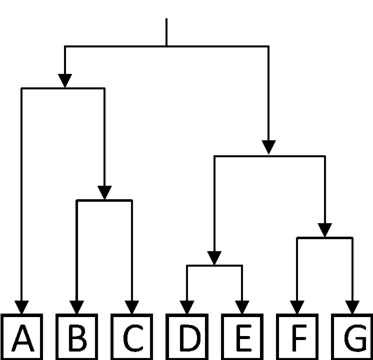
\includegraphics[width=0.40\textwidth]{hierarchical-clustering-example2}
    \caption{}
	%\caption{Hierarchical clustering example. The partial relation exists only between clusters.} 
	\label{fig:hierarchical-example} 
  \end{subfigure}%
  ~
  \begin{subfigure}[t]{0.5\textwidth}
  	\centering
    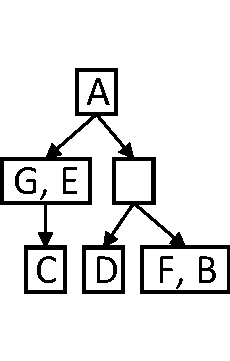
\includegraphics[width=0.40\textwidth, trim={0 1.15cm 0 1.15cm}, clip]{OCH-clustering-example}
    \caption{}
	%\caption{Object Cluster hierarchy example. The partial relation exists between both the clusters and the objects.}
	 \label{fig:och-example} 
  \end{subfigure}
  \caption{Dendrogram (a) and Object Cluster Hierarchy (b) examples. Letters represent objects and squares are groups. The arrows show the partial order relation. In the Dendrogram, the partial relation exists between both the clusters and the objects, whereas in the Object Cluster Hierarchy the partial relation exists between both the clusters and the objects.}
\end{figure}
    
The OCH approach extends HC by allowing objects to be assigned to any node of the hierarchy tree. Researchers have developed methods with such capability, which is enough to receive a new hierarchy relation that exists between objects, e.g.,~\cite{ghahramani2010tree,2010_bayesian_rose_trees,Spytkowski2012,Olech2016}.

    Within this paradigm we have formulated three important requirements~\cite{Spytkowski2012} to accurately reflect a semantic (ontological) approach to Hierarchical Clustering:
\begin{enumerate}
    \item {\textit{Inheritance} -- every object belonging to a given group also belongs to the parents groups, up to the root;}
    \item {\textit{Retention} -- objects are not required to be located in the tree’s leaves;}
    \item {\textit{Variance} -- groups located lower in the hierarchy are more specific, i.e., every child group has to have not higher variation than its parents.}
\end{enumerate}

These formal requirements serve to closer reflect the human perception of hierarchy that can be also found in images~\cite{ILSVRC15,ghahramani2010tree}, documents~\cite{ghahramani2010tree,2010_bayesian_rose_trees}, and communities structure~\textbf{lancichinetti2009detecting<- cos nowszego, massaro2014hierarchical}.

In \Cref{fig:och-example} a comparison between Hierarchical Clustering (a) and Object Cluster Hierarchy (b) is presented. In the former, the final clustering is flat, and the number of clusters depends on the hight where the Dendrogram is cut. Considering~\Cref{fig:hierarchical-example}, by cutting the tree at the bottom of the hierarchy, a set of seven clusters is formed, each of them containing one letter. Regardless of where the hierarchy is cut, the resulting clustering consists of all the same seven letters. In comparison, in \Cref{fig:och-example}, the whole OCH represents the clustering - partition of all 7 letters. There is no need to cut a hierarchy. Due to hierarchical relations, objects from child clusters conceptually belongs to the parent clusters. Root always contains all the objects (i.e., the whole set), whereas leaves contain only what belongs to them.

A hierarchy with data points placed in leaves only is a valid OCH thus all the HC results are always a OCH, but the opposite does not always hold true due to the \textit{Retantion} requirement. Hierarchical Clustering result always contain all the data points at the bottom of the hierarchy. Thus, OCH is an abstraction over Hierarchical Clustering.

Object Cluster Hierarchy is a novel concept that is recently gaining more interest. One of the first works on the subject of Object Clusters Hierarchy was published in~\cite{ghahramani2010tree} where the authors pointed out that many data arise from a latent hierarchy, for example, a set of text documents or images. Such data can be modelled by an Object Cluster Hierarchy, which is one possible way to discover the unobservable structure by inferring it during a learning process. Authors in~\cite{ghahramani2010tree} proposed a nonparametric method allowing to develop trees of unbounded width and depth. The objects can be assigned to any node in a created tree. Thus, some nodes can be empty, i.e., without any objects assigned. This method does not satisfy the \textit{Variance} requirement. Objects belonging to the child node can vary more than objects assigned to its parent node. Starting from this method as the prototype, the ongoing development has been carried out to propose a new version of it. The first prototype of it was presented in~\cite{Spytkowski2016}.

    During the development of the method mentioned above, the authors met troubles with comparing the new method with others, especially with the inspiration~\cite{ghahramani2010tree} and Bayesian Rose Trees~\cite{DBLP:journals/corr/abs-1203-3468}. The problem, to the best of our knowledge, is twofold: firstly, there are no appropriate evaluation measures dedicated to object cluster hierarchies which would reflect the desired properties listed above. Secondly, there are no available benchmark datasets with known properties, which could be used for testing different methods of hierarchical structure generation.
    
We started with a partial solution to the first problem that is presented in~\cite{Spytkowski2016}. However, new external and internal validation techniques have been developed and are planned to be published soon as their experimental study requires appropriate datasets. That requirement led to a development of a method generating the data structures with known characteristics that is addressed in this article. Being able to model the characteristics of created artificial datasets allows more in-depth analysis of both methods and evaluation measures.
%
\section{Generator model}
\label{model}
	The data generated by this model	 can be seen as data coming from an infinite mixture model. Most commonly an infinite mixture model is composed of infinite, indexed distributions from which the data is drawn. In such case the mixture weights can be drawn from a Dirichlet distribution, using the Stick Breaking Process. Generally, the distributions for the mixture components are unrelated to each other. This generator uses a similar approach, however, it bases its mixture weights on the Tree-Structured Stick Breaking Process, as described in~\cite{ghahramani2010tree}, which arranges the mixture components into a hierarchical structure. This structure also defines the relationship between the mixture components, that is -- children distributions are based on their parent's parameters.
    
    Hierarchies generated using the Stick Breaking Process posses the following characteristics~\cite{ghahramani2010tree, Spytkowski2012}:
\begin{enumerate}
    \item Every node can have an infinite number of child nodes;
    \item The children of a node are indexed and ordered. However, this indexing is not important after the generation process finishes;
    \item Every node in the hierarchy can have child nodes, the potential depth of the hierarchy is not limited to any crisp value;
    \item The hierarchy may contain empty nodes, that is, the nodes that do not generate any data;
    \item The child node distribution parameters are generated based on the parent parameters and a kernel describing the transition;
    \item The shape of the generated hierarchy depends on a number of control hyperparameters described in the~\cref{parameter}.
\end{enumerate}
    
    Throughout this paper following symbols are used to describe the generator and the generated model:
	%
\begin{tabbing}
	$X$ \hspace{10mm} \= - set of all data points, or objects, \\
	$x_i$ \> - an object or data point with unique identifier\\ \> $i$ represented by a vector of features, \\
	$\Theta$ \> - set of all clusters, \\
	$\epsilon$ \> - specific cluster from $\Theta$, \\
	$\epsilon_{x_i}$ \> - cluster of object $x_i$, \\
	$\epsilon\epsilon_i$ \> - the $i-th$ child of cluster $\epsilon$, if the Object Cluster Hierarchy is defined\\
	$\epsilon_\varnothing$ \> - the root cluster of the Object Cluster Hierarchy\\
	$X_\epsilon$ \> - set of all objects in cluster $\epsilon$, \\
	$X_{E_\epsilon}$ \> - set of all objects in hierarchy subtree\\ \> starting with node $\epsilon$, \\
	$|S|$ \> - number of elements in set S, \\
	$|\epsilon|$ \> - depth of a node $\epsilon$, \\
	$\theta_\epsilon$ \> - data distribution for the node $\epsilon$. Specifically, $\theta_{\epsilon_\varnothing}$ is the distribution of \\ \> the root node,  $\theta_{\epsilon_c}$ is the distribution of a node $\epsilon_c$, and $\theta_{\epsilon\epsilon_i}$ is the \\ \> distribution of a $i-th$ child of cluster $\epsilon$, \\
	$Beta(\alpha, \beta)$ \; - Beta distribution with shape parameters $\alpha$ and $\beta$, \\
	$Gauss(\mu, \sigma)$ \; - Gaussian distribution with mean $\mu$ and standard deviation $\sigma$.
\end{tabbing}	
	Additionally to the symbols above, several values are provided to the generator as parameters. The use of these parameters is further described in the~\cref{parameter} and their influence on the final result is empirically shown in the~\cref{experiments}:
%
\begin{tabbing}
	$d$ \hspace{10mm} \= - the dimensionality of the generated data points, \\
	$n$ \> - the number of data points to be generated, \\
	$\alpha_0, \lambda$ \> - input parameters controlling the hierarchy\\ \> depth, used by equation $\alpha(\epsilon) = \alpha_0\lambda^{|\epsilon|}$ \\
	$\gamma$ \> - parameter controlling the width of a tree structure, \\
	$p, q$ \> - parameters controlling the specificity of the generated data. \\ \> They influence how much smaller the deviation of points'  \\ \> features in the child node should be in comparison with \\ \> points in the parent node, \\
	$\theta_{\epsilon_\varnothing}$ \> - the distribution of the root node.
\end{tabbing}
	
	Having these parameters we can defining the generator itself. We start with the conditional probabilities used to determine which node data is generated from. The first is the conditional probability of a datum remaining in node $\epsilon$, at depth $|\epsilon|$, when entering the node:
%
\begin{equation}
\nu_\epsilon = P(x \in X_\epsilon | x \in X_{E_\epsilon}),
\end{equation}
%
\begin{equation}\label{eq:alpha_function}
\nu_\epsilon \sim Beta(1, \alpha(\epsilon)),\;\;\; \alpha(\epsilon) = \alpha_0\lambda^{|\epsilon|}.
\end{equation}
	%
	The second is the conditional probability of a datum being transferred to the subtree $\epsilon\epsilon_i$ if it does not remain in node $\epsilon$ and hasn't been transferred to any of the previous siblings (i.e., did not travel down sibling subtrees with a lower indices $\epsilon\epsilon_j,~j < i$): 

%
\begin{equation}
\begin{multlined}
\psi_{\epsilon\epsilon_i} = P(x \in X_{E_{\epsilon\epsilon_i}} | x \in X_{E_\epsilon} \wedge  x \not\in X_\epsilon \wedge \neg \exists_{j < i} x \in X_{E_{\epsilon\epsilon_j}}),
\end{multlined}
\end{equation}
%
\begin{equation}
\psi_{\epsilon\epsilon_i} \sim Beta(1, \gamma).
\end{equation}
%
	Additionally, we need to define the kernel. We begin with a specified root node distribution $\theta_{\epsilon_\varnothing}$ given as a starting parameter of the generation method. The values set at this point are the means $(\mu)$ and standard deviations $(\sigma)$ for each of the $Gauss$ distributions in the $d$ different dimensions:
%
\begin{equation}
\label{eq:theta-epsilon-varnothing}
\theta_{\epsilon_\varnothing} = (Gauss(\mu_{{\epsilon_\varnothing} 1}, \sigma_{{\epsilon_\varnothing} 1}), ... , Gauss(\mu_{{\epsilon_\varnothing} d}, \sigma_{{\epsilon_\varnothing} d})).
\end{equation}
	From there, for any node for which we need the distribution, we can draw the distribution based on the parent's distribution. The child's mean values are drawn directly from the parent distribution, and the child's standard deviation is based on a scaling factor ($\Delta\sigma_n$) drawn from a $Beta$ distribution. The values are taken separately for each dimension:
	%
	\begin{equation}
    \label{eq:theta-epsilon-epsilon-i}
	\begin{multlined}
	\theta_{\epsilon\epsilon_i} = (Gauss(\Delta\mu_1, \sigma_{\epsilon 1} \Delta\sigma_1), ... , Gauss(\Delta\mu_d, \sigma_{\epsilon d} \Delta\sigma_d)),
	\end{multlined}
	\end{equation}
	%
	\begin{equation}
    \label{eq:delta-miu-n}
	\Delta\mu_n \sim Gauss(\mu_{\epsilon n}, \sigma_{\epsilon n}), \;\;\;n = 1 ... d,
	\end{equation}
	
	\begin{equation}
    \label{eq:delta-sigma-n}
	\Delta\sigma_n \sim Beta(p, q), \;\;\;n = 1 ... d.
	\end{equation}
	%
	With the kernel defined we can now generate data from the model. We begin with the hyperparameters and the probability distribution for the root node ($\theta_{\epsilon_\varnothing} = (Gauss(\mu_{\epsilon_\varnothing 1}, \sigma_{\epsilon_\varnothing 1}), ..., Gauss(\mu_{\epsilon_\varnothing d}, \sigma_{\epsilon_\varnothing d}))$).
	
	The following process continues until we generate $n$ points:
	
	\noindent\textbf{Step 1:} If $|X| < n$ go to \textbf{Step2}, else \textbf{end}.\\
	%
	\textbf{Step 2:} Randomly draw an insertion point $i_x \sim Uni(0, 1)$, $i_x \in (0, 1)$.\\
	%
	\textbf{Step 3:} Set the root node as the current node ($\epsilon_c := \epsilon_\varnothing$), depth is 0 ($|\epsilon_c| := 0$).\\
	%
	\textbf{Step 4:} If $\nu$ for the current node is not yet known, draw the value. $\nu_{\epsilon_c} \sim Beta(1, \alpha_0 \lambda ^ {|\epsilon_c|} )$.\\
	%
	\textbf{Step 5:} If $i_x \leq \nu_{\epsilon_c}$ then $x \sim \theta_{\epsilon_c}$ ($x \sim \theta_{\epsilon_\varnothing}$ if $\epsilon_c = \epsilon_\varnothing$), the point belongs to the current node ($X_{\epsilon_c} := \{x\} \cup X_{\epsilon_c}$), go to \textbf{Step 1}, else move on to \textbf{Step 6}.\\
	%
	\textbf{Step 6:} Adjust $i_x$ to new value: $i_x := (i_x - \nu_{\epsilon_c}) / (1 - \nu_{\epsilon_c})$.\\
	%
	\textbf{Step 7:} Set current child node index ($\epsilon_c\epsilon_i$) to the first child node of the current node: $i := 0$.\\
	%
	\textbf{Step 8:} If $\psi$ for the current child node is not yet known, draw the value: $\psi_{\epsilon_c\epsilon_i} \sim Beta(1, \gamma)$.\\
	%
	\textbf{Step 9:} If $\theta_{\epsilon_c\epsilon_i}$ for the current child node is not yet known, draw the values based on the parent of the node: 
	\noindent	
	$\theta_{\epsilon_c\epsilon_i} = (Gauss(\Delta\mu_1, \sigma_{\epsilon_c 1} \Delta\sigma_1), ..., Gauss(\Delta\mu_d, \sigma_{\epsilon_c d}\Delta\sigma_d))$,
	\noindent
	$\Delta\mu_1$ is drawn from the first dimension of parent node ($\Delta\mu_1 \sim Gauss(\mu_{\epsilon_c 1}, \sigma_{\epsilon_c 1})$),
	\noindent		
	...
	\noindent		
	$\Delta\mu_d$ is drawn from $d$-th dimension of parent node ($\Delta\mu_d \sim Gauss(\mu_{\epsilon_c d}, \sigma_{\epsilon_c d})$),
	\noindent		
	$\Delta\sigma_1\sim Beta(p, q)$,
	\noindent		
	...
	\noindent		
	$\Delta\sigma_d\sim Beta(p, q)$.\\
	%
	\textbf{Step 10:} If $i_x \leq \psi_{\epsilon_c\epsilon_i}$ go to \textbf{Step 11}, else go to \textbf{Step 12}.\\
	%
	\textbf{Step 11:} Adjust the value of $i_x$ to new value: $i_x := i_x / \psi_{\epsilon_c\epsilon_i}$. Make the current child the current node ($\epsilon_c := \epsilon_c\epsilon_i$) and increase depth ($|\epsilon_c| := |\epsilon_c| + 1$). Go to \textbf{Step 4}.\\
	%
	\textbf{Step 12:} Adjust the value of $i_x$ to new value $i_x := (i_x - \psi_{\epsilon_c\epsilon_i}) / (1 - \psi_{\epsilon_c\epsilon_i})$. Increment child index of currently relevant child node ($i: = i + 1$). Go to \textbf{Step 8}.
	
	For better understanding, the generation process described above is illustrated in the block diagram, in Figure~\ref{fig:generator-block-diagram}.
	%
	\noindent
\begin{figure*}[h]
  \begin{center}
    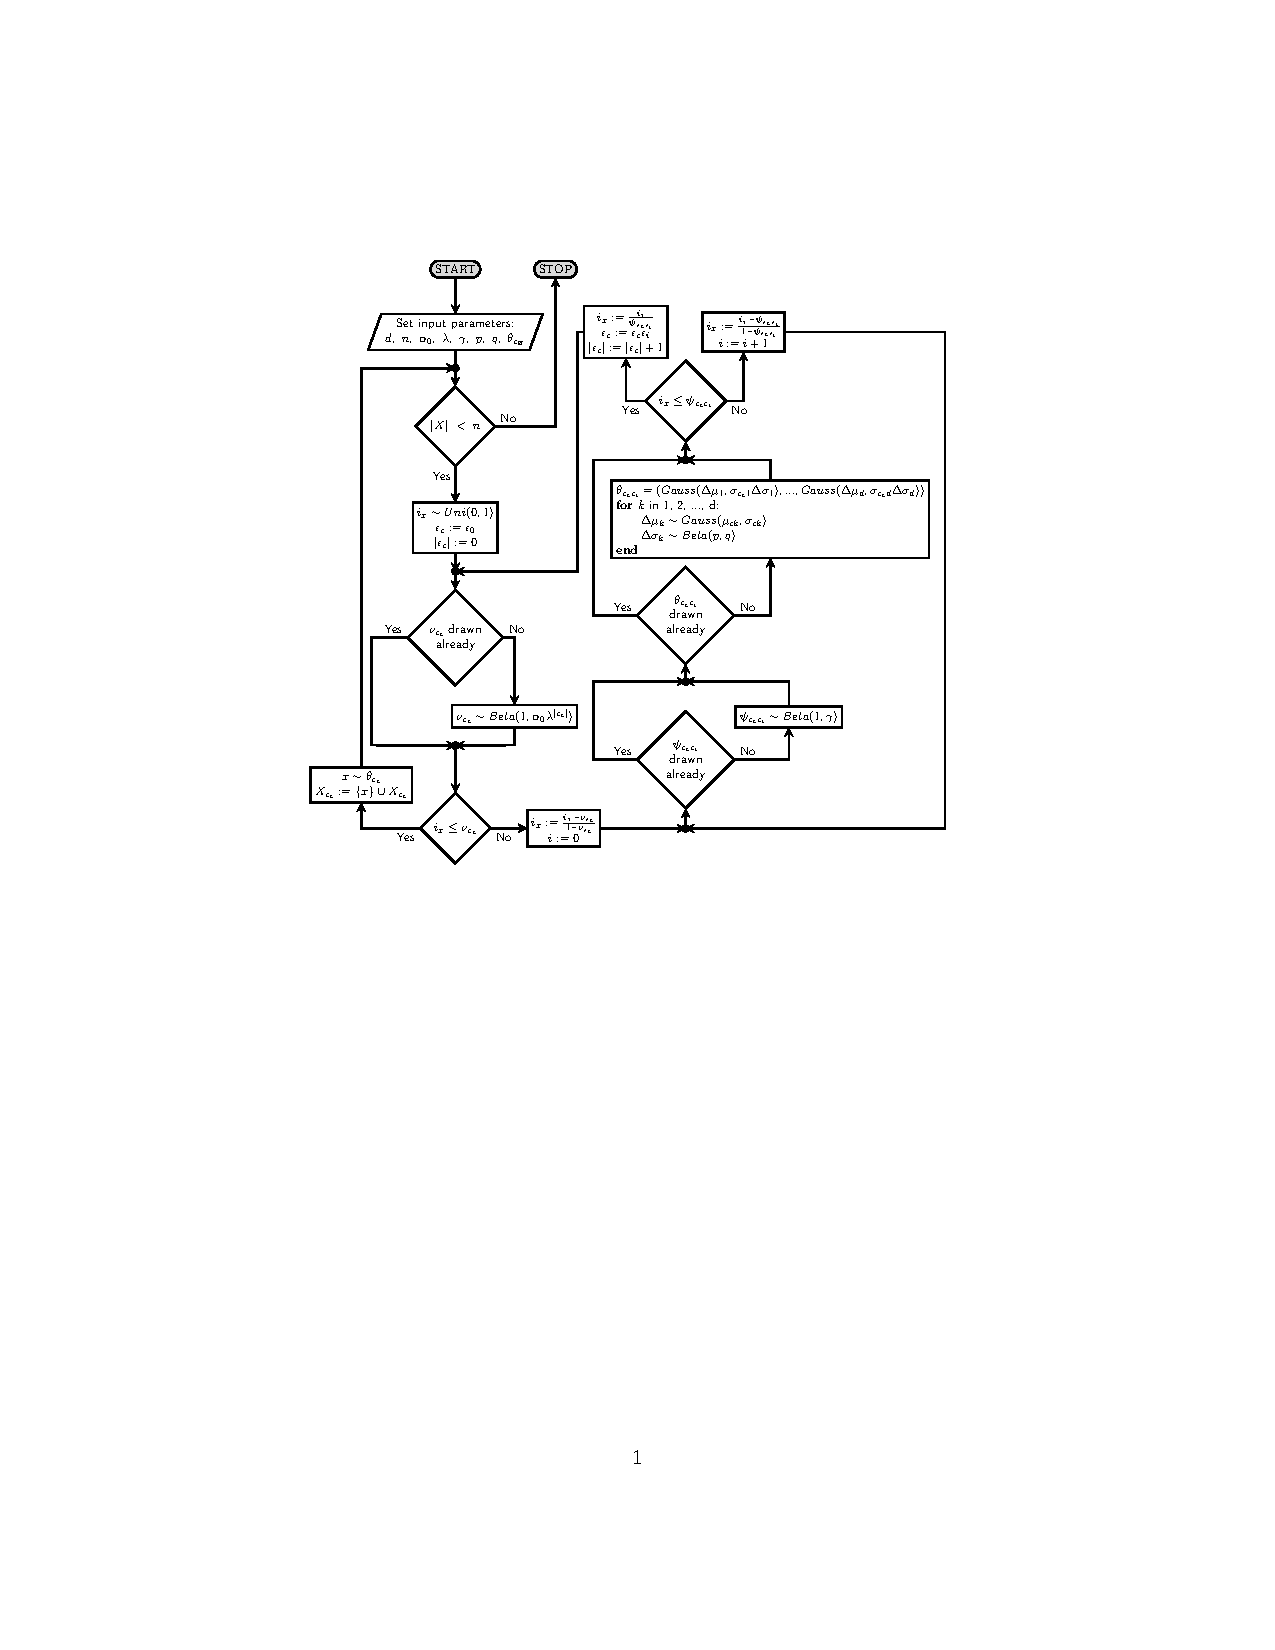
\includegraphics[clip, trim=5.2cm 13.3cm 5.4cm 4.4cm, width=0.75\textwidth]{generator-block-diagram}
	\caption{Block diagram of Object Cluster Hierarchy generator.} \label{fig:generator-block-diagram} 
  \end{center}
\end{figure*}
	%
	\section{Parameter selection}
	\label{parameter}    
    Hierarchical data might follow hierarchies of different characteristics, e.g., number of objects, depth, width. Thus, to provide the best possible benchmarks for all problems, the generator should provide a high flexibility in generating a variety of hierarchies. The primary interest is in the structure of the hierarchy, that is if the hierarchy is tall or short, wide or narrow, as well as the distribution of data across the levels of the hierarchy. Additionally, the difference between data in parent and child nodes can also be important in some cases. All of these are controlled by a number of parameters in the model:
	%
	\begin{enumerate}
		\item hierarchy depth: $\alpha_0$, $\lambda$ or in a more general sense -- the $\alpha(\epsilon)$ function,
		\item hierarchy width: $\gamma$,
		\item data specificity: $p$, $q$,
		\item starting node distribution: $\theta_{\epsilon_\varnothing}$.
	\end{enumerate}
	%
	\subsection{Controlling the hierarchy depth}
    \label{sec:controlling-the-hierarchy-depth}
	%
	The depth of the hierarchy is controlled by the parameters $\alpha$. The higher the probabilities of data remaining in nodes, the fewer data will travel deep down the tree, and thus the tree will be shallower. On the other hand, if the probability is low, the data will, on average, travel deeper into the tree before stopping. The average probability of data remaining in a given node is based on the selected $\alpha$ function, which in turn is the basis for estimating the behaviour of the tree based on the $\alpha_0$ and $\lambda$ parameters:
	%
	\begin{equation}
	\mathbf{E}[x \in X_\epsilon, |\epsilon| = 0] = \frac{1}{1 + \alpha_0},
	\end{equation}
	\begin{equation}
	\mathbf{E}[x \in X_\epsilon, |\epsilon| = n] = \frac{\prod_{i=0}^{n-1} \alpha_0\lambda^i}{\prod_{j=0}^{n}(1 + \alpha_0\lambda^j)}.
	\end{equation}
	%
	Additionally the variance can also be calculated:
	%
	\begin{equation}
	\mathbf{var}[x \in X_\epsilon, |\epsilon| = 0] = \frac{\alpha_0}{(1 + \alpha_0)^2(2 + \alpha_0)},
	\end{equation}
	\begin{equation}
	\begin{multlined}
	\mathbf{var}[x \in X_\epsilon, |\epsilon| = n] = \\ = \frac{2 \prod_{i = 0}^{n-1}\alpha_0\lambda^i}{(1+\alpha_0\lambda^n)\prod_{j=0}^{n}(2+\alpha_0\lambda^j)} \\ - \left(\textbf{E}[x \in X_\epsilon, |\epsilon| = n]\right)^2.
	\end{multlined}
	\end{equation}
	%
	Taking $\alpha(\epsilon)$ and $\gamma$, as well as the data generation procedure, it is possible to estimate the shape of the tree:
    %
    \begin{itemize}
        \item $\alpha_0 = 1, \lambda = 1$: The structure of the tree is chaotic and hard to predict, the further away the parameters move from these values the more stable the tree becomes;
        \item $\alpha_0 < 1, \lambda \leq 1$: Shallow structure, data located primarily at the top of the tree;
        \item $\alpha_0 < 1, \lambda > 1$: Similar to the above case, the depth of the tree increases but most data is located at the top of the tree;
        \item $\alpha_0 > 1, \lambda < 1$: The structure is deep, but data is not located at the top, the bigger $\alpha_0$ starts out, and smaller $\lambda$ is the more data will move down the tree into the central or lower region;
        \item $\alpha_0 > 1, \lambda \geq 1$: Deep structure, data located primarily at the top of the tree but spread out.
    \end{itemize}
    \subsection{Controlling the hierarchy width}
    %
    The width of the tree is based on the value of the $\gamma$ parameter at a given node depth $j$. Given that 
    $x \in X_{E_\epsilon}$ and $x \not \in X_\epsilon$ the average probability of data being generated from a specific subtree (based on the index) can be used to estimate the number of children a node can potentially have:
	%
    \begin{equation}
    \mathbf{E}[x \in X_{E_{\epsilon\epsilon_i}}, i = 1] = \frac{1}{1 + \gamma},
    \end{equation}
	
    \begin{equation}
    \mathbf{E}[x \in X_{E_{\epsilon\epsilon_i}}, i = n] = \frac{\gamma^{n-1}}{(1 + \alpha_0\lambda^j)^n}.
    \end{equation}
	%
	Variance for these values can also be calculated:
	%
    \begin{equation}
	\mathbf{var}[x \in X_{E_{\epsilon\epsilon_i}}, i = 1] = \frac{\gamma}{(1 + \gamma)^2(2 + \gamma)},
	\end{equation}
	
    \begin{equation}
	\begin{multlined}
	\mathbf{var}[x \in X_{E_{\epsilon\epsilon_i}}, i = n] = \frac{2 \gamma^{n-1}}{(1+\gamma)(2+\gamma)^n} - \left(\textbf{E}[x \in X_{E_{\epsilon\epsilon_i}}, i = n]\right)^2.
	\end{multlined}
	\end{equation}
	%
	Once more, taking the generation procedure into account and the influence of the parameter on the estimated values to judge the general tendencies of the model:
	%
	\begin{itemize}
		\item $\gamma = 1$: The number of children is chaotic and difficult to judge;
		\item $\gamma < 1$: Narrower tree, less children per node on average;
		\item $\gamma > 1$: Wider tree, more children per node on average.
	\end{itemize}
	Additionally, these tendencies were empirically shown in the~\cref{experiments}. 
	%
	\subsection{Controlling data specificity}
	%
	When a new group is considered, the parameters for that group's distribution are drawn based on the parent distribution and the $p$ and $q$ kernel parameters. An important aspect of the generated model is that data becomes more specific in lower nodes. This behaviour is always present, however, the values taken for the kernel change the average proportion 
    %between data standard deviation between the parent and child. 
    of standard data deviation between the parent and child.
    This is based on the expected standard deviation of the new node compared to the old node (taken separately in each dimension):
	%
	\begin{equation}\label{eq:analitical_expected_standard_dev}
	\mathbf{E}[\sigma_{\epsilon\epsilon_id}] = \sigma_{\epsilon d} \frac{p}{p + q},
	\end{equation}
	%
	\begin{equation}\label{eq:analitical_variance_standard_dev}
	\mathbf{var}[\sigma_{\epsilon\epsilon_id}] = \sigma_{\epsilon d} \frac{pq}{(p + q)^2(p + q + 1)}.
	\end{equation}
	%
	By selecting $p$ and $q$ the rate at which the nodes become more specific can be altered. The lower the mean is, the more specific every child will be (on average), the higher the variance is, the more variety there will be in how the child nodes relate to their parent.
	%
	\subsection{Influence of starting distribution on results}
	%
	Due to the relative nature of the model (i.e., the specific values generated from the model are calculated relative to each other, starting from the root distribution, as shown in equations~\ref{eq:theta-epsilon-varnothing},~\ref{eq:theta-epsilon-epsilon-i},~\ref{eq:delta-miu-n},~\ref{eq:delta-sigma-n}) the choice of initial distribution parameters is not important. The data generated from the model can be scaled afterwards to any desired values as well as moved in any direction along any dimension. Due to this, the generator assumes a value for $\theta_{\epsilon_\varnothing}$:
	%
    \begin{equation}
	\theta_{\epsilon_\varnothing} = (Gauss(0,\sigma_{max}), ..., Gauss(0,\sigma_{max})).
	\end{equation}
	%
	Every dimension of the root node is described by a normal distribution with $\mu_{{\epsilon_\varnothing} 1} = \mu_{{\epsilon_\varnothing} 2} = ... = \mu_{{\epsilon_\varnothing} d} = 0$ and the standard deviation of value $\sigma_{max}$ which is a method's parameter. Within our experiments $\sigma_{max} = 10$. Data generated from the model can be then post-processed to a more desirable spread of values. This is done by applying scaling and translation to all the data generated by the model as well as the parameters of each group node.
	%
	\subsection{Post-processing}
	%
	The data also undergoes one form of post-processing after being generated. This process, referred in this paper as \textit{reassignment}, moves the data between clusters in such a way that each object belongs to the cluster it is most likely to be generated by:
	%
	\begin{equation}
	\forall_{x \in X}\left( x \in X_{\epsilon_a}\Leftrightarrow \neg\exists_{\epsilon_b \neq \epsilon_a}L(x|\theta_{\epsilon_a})<L(x|\theta_{\epsilon_b})\right )
	\end{equation}
	%
	The process does not modify the clusters number, relations or parameters in any way. It merely relocates data to reduce noise and produce cleaner clusters.
	%%%%%%%%%%%%%%%%%%%%%%%%%%%%%%%%%%%%%%%%%%%%%%%%%%%%%%%%%%%%%%%%%%%%%%%%%%%%%%%%%%%%%%%%%%%%%%%%%%%%%%%%%%%%%%
    \noindent
\begin{figure*}[p!]
\centering
\begin{tabular}{rrrr}
%%%%%%%%%%%%%%%%%%%%%%%%%%%%%%%%%%%%%%%%%%%%%%%%%%%%%
  \begin{tikzpicture}
    \begin{axis} 
		[
	  	ybar,
	  	title=s00,
		  xmin = -0.5,
		  xmax = 6.5,
		  bar width = 11.6,
		]
		\addplot
		[
			color = blue,
			fill = blue,
		]
		table
		[
	  	col sep = semicolon,
	  	x = "Level",
	  	y = "s00",
		]
		{avgHierarchyWidthPerLevel.csv};
		\end{axis}
  \end{tikzpicture}&%
%%%%%%%%%%%%%%%%%%%%%%%%%%%%%%%%%%%%%%%%%%%%%%%%%%%%%
  \begin{tikzpicture}
    \begin{axis} 
		[
	  	ybar,
	  	title=s01,
		  xmin = -0.6,
		  bar width = 4.2,
		]
		\addplot
		[
			color = blue,
			fill = blue,
		]
		table
		[
	  	col sep = semicolon,
	  	x = "Level",
	  	y = "s01",
		]
		{avgHierarchyWidthPerLevel.csv};
		\end{axis}
  \end{tikzpicture}&%
%%%%%%%%%%%%%%%%%%%%%%%%%%%%%%%%%%%%%%%%%%%%%%%%%%%%%
  \begin{tikzpicture}
    \begin{axis} 
		[
	  	ybar,
	  	title=s02,
		  xmin = -0.55,
		  bar width = 4.4,
		]
		\addplot
		[
			color = blue,
			fill = blue,
		]
		table
		[
	  	col sep = semicolon,
	  	x = "Level",
	  	y = "s02",
		]
		{avgHierarchyWidthPerLevel.csv};
		\end{axis}
  \end{tikzpicture}&%
%%%%%%%%%%%%%%%%%%%%%%%%%%%%%%%%%%%%%%%%%%%%%%%%%%%%%
  \begin{tikzpicture}
    \begin{axis} 
		[
	  	ybar,
	  	title=s03,
		  xmin = -0.5,
		  xmax = 8.5,
	   	bar width = 9.0,
		]
		\addplot
		[
			color = blue,
			fill = blue,
		]
		table
		[
	  	col sep = semicolon,
	  	x = "Level",
	  	y = "s03",
		]
		{avgHierarchyWidthPerLevel.csv};
		\end{axis}
  \end{tikzpicture}\\%
%%%%%%%%%%%%%%%%%%%%%%%%%%%%%%%%%%%%%%%%%%%%%%%%%%%%%
  \begin{tikzpicture}
    \begin{axis} 
		[
	  	ybar,
	  	title=s04,
		  xmin = -0.5,
		  bar width = 0.8,
		]
		\addplot
		[
			color = blue,
			fill = blue,
		]
		table
		[
	  	col sep = semicolon,
	  	x = "Level",
	  	y = "s04",
		]
		{avgHierarchyWidthPerLevel.csv};
		\end{axis}
  \end{tikzpicture}&%
%%%%%%%%%%%%%%%%%%%%%%%%%%%%%%%%%%%%%%%%%%%%%%%%%%%%%
  \begin{tikzpicture}
    \begin{axis} 
		[
	  	ybar,
	  	title=s05,
		  xmin = -0.45,
		  xmax = 9.3,
		  bar width = 8.1,
		]
		\addplot
		[
			color = blue,
			fill = blue,
		]
		table
		[
	  	col sep = semicolon,
	  	x = "Level",
	  	y = "s05",
		]
		{avgHierarchyWidthPerLevel.csv};
		\end{axis}
  \end{tikzpicture}&%
%%%%%%%%%%%%%%%%%%%%%%%%%%%%%%%%%%%%%%%%%%%%%%%%%%%%%
  \begin{tikzpicture}
    \begin{axis} 
		[
	  	ybar,
	  	title=s06,
		  xmin = -0.5,
		  xmax = 10.6,
		  bar width = 7.1,
		]
		\addplot
		[
			color = blue,
			fill = blue,
		]
		table
		[
	  	col sep = semicolon,
	  	x = "Level",
	  	y = "s06",
		]
		{avgHierarchyWidthPerLevel.csv};
		\end{axis}
  \end{tikzpicture}&%
%%%%%%%%%%%%%%%%%%%%%%%%%%%%%%%%%%%%%%%%%%%%%%%%%%%%%%
  \begin{tikzpicture}
    \begin{axis} 
		[
	  	ybar,
	  	title=s07,
		  xmin = -0.5,
		  xmax = 11.6,
		  bar width = 6.5,
		]
		\addplot
		[
			color = blue,
			fill = blue,
		]
		table
		[
	  	col sep = semicolon,
	  	x = "Level",
	  	y = "s07",
		]
		{avgHierarchyWidthPerLevel.csv};
		\end{axis}
  \end{tikzpicture}
%%%%%%%%%%%%%%%%%%%%%%%%%%%%%%%%%%%%%%%%%%%%%%%%%%%%%%
\end{tabular}
\caption{Average hierarchy width $(B)$ on every hierarchy level (number of nodes on every level) \textbf{without} execution of reassignment procedure. Vertical axes show hierarchy width and horizontal axes indicate hierarchy level.}\label{fig:level-by-level-hierarchy-width}
\end{figure*}
%%%%%%%%%%%%%%%%%%%%%%%%%%%%%%%%%%%%%%%%%%%%%%%%%%%%%%%%%%%%%%%%%%%%%%%%%%%%%%%%%%%%%%%%%%%%%%%%%%%%%%%%%%%%%%
\noindent
\begin{figure*}[p!]
\centering
\begin{tabular}{rrrr}
%%%%%%%%%%%%%%%%%%%%%%%%%%%%%%%%%%%%%%%%%%%%%%%%%%%%%
  \begin{tikzpicture}
    \begin{axis} 
		[
	  	ybar,
	  	title=s00,
		  xmin = -0.5,
		  xmax = 6.5,
		  bar width = 11.5,
		]
		\addplot
		[
			color = blue,
			fill = blue,
		]
		table
		[
	  	col sep = semicolon,
	  	x = "Level",
	  	y = "s00r",
		]
		{avgHierarchyWidthPerLevel.csv};
		\end{axis}
  \end{tikzpicture}
  &
%%%%%%%%%%%%%%%%%%%%%%%%%%%%%%%%%%%%%%%%%%%%%%%%%%%%%
  \begin{tikzpicture}
    \begin{axis} 
		[
	  	ybar,
	  	title=s01,
		  xmin = -0.6,
		  bar width = 4.1,
		]
		\addplot
		[
			color = blue,
			fill = blue,
		]
		table
		[
	  	col sep = semicolon,
	  	x = "Level",
	  	y = "s01r",
		]
		{avgHierarchyWidthPerLevel.csv};
		\end{axis}
  \end{tikzpicture}
  &
%%%%%%%%%%%%%%%%%%%%%%%%%%%%%%%%%%%%%%%%%%%%%%%%%%%%%
  \begin{tikzpicture}
    \begin{axis} 
		[
	  	ybar,
	  	title=s02,
		  xmin = -0.55,
		  bar width = 4.4,
		]
		\addplot
		[
			color = blue,
			fill = blue,
		]
		table
		[
	  	col sep = semicolon,
	  	x = "Level",
	  	y = "s02r",
		]
		{avgHierarchyWidthPerLevel.csv};
		\end{axis}
  \end{tikzpicture}
  &
%%%%%%%%%%%%%%%%%%%%%%%%%%%%%%%%%%%%%%%%%%%%%%%%%%%%%
  \begin{tikzpicture}
    \begin{axis} 
		[
	  	ybar,
	  	title=s03,
		  xmin = -0.5,
		  xmax = 8.5,
	   	bar width = 8.8,
		]
		\addplot
		[
			color = blue,
			fill = blue,
		]
		table
		[
	  	col sep = semicolon,
	  	x = "Level",
	  	y = "s03r",
		]
		{avgHierarchyWidthPerLevel.csv};
		\end{axis}
  \end{tikzpicture}
  \\
%%%%%%%%%%%%%%%%%%%%%%%%%%%%%%%%%%%%%%%%%%%%%%%%%%%%%
  \begin{tikzpicture}
    \begin{axis} 
		[
	  	ybar,
	  	title=s04,
		  xmin = -0.5,
		  bar width = 0.8,
		]
		\addplot
		[
			color = blue,
			fill = blue,
		]
		table
		[
	  	col sep = semicolon,
	  	x = "Level",
	  	y = "s04r",
		]
		{avgHierarchyWidthPerLevel.csv};
		\end{axis}
  \end{tikzpicture}
  &
%%%%%%%%%%%%%%%%%%%%%%%%%%%%%%%%%%%%%%%%%%%%%%%%%%%%%
  \begin{tikzpicture}
    \begin{axis} 
		[
	  	ybar,
	  	title=s05,
		  xmin = -0.45,
		  xmax = 9.3,
		  bar width = 8.1,
		]
		\addplot
		[
			color = blue,
			fill = blue,
		]
		table
		[
	  	col sep = semicolon,
	  	x = "Level",
	  	y = "s05r",
		]
		{avgHierarchyWidthPerLevel.csv};
		\end{axis}
  \end{tikzpicture}
  &
%%%%%%%%%%%%%%%%%%%%%%%%%%%%%%%%%%%%%%%%%%%%%%%%%%%%%
  \begin{tikzpicture}
    \begin{axis} 
		[
	  	ybar,
	  	title=s06,
		  xmin = -0.5,
		  xmax = 10.6,
		  bar width = 7.1,
		]
		\addplot
		[
			color = blue,
			fill = blue,
		]
		table
		[
	  	col sep = semicolon,
	  	x = "Level",
	  	y = "s06r",
		]
		{avgHierarchyWidthPerLevel.csv};
		\end{axis}
  \end{tikzpicture}
  &
  %%%%%%%%%%%%%%%%%%%%%%%%%%%%%%%%%%%%%%%%%%%%%%%%%%%%%%
  \begin{tikzpicture}
    \begin{axis} 
		[
	  	ybar,
	  	title=s07,
		  xmin = -0.5,
		  xmax = 11.6,
		  bar width = 6.5,
		]
		\addplot
		[
			color = blue,
			fill = blue,
		]
		table
		[
	  	col sep = semicolon,
	  	x = "Level",
	  	y = "s07r",
		]
		{avgHierarchyWidthPerLevel.csv};
		\end{axis}
  \end{tikzpicture}
%%%%%%%%%%%%%%%%%%%%%%%%%%%%%%%%%%%%%%%%%%%%%%%%%%%%%%
\end{tabular}
\caption{Average hierarchy width $(B)$ on every hierarchy level (number of nodes on every level) \textbf{with} execution of reassignment procedure. Vertical axes show hierarchy width and horizontal axes indicate hierarchy level.}\label{fig:level-by-level-hierarchy-width-R}
\end{figure*} %2
	\noindent
\begin{figure*}[p!]
\centering
\begin{tabular}{llll}
%%%%%%%%%%%%%%%%%%%%%%%%%%%%%%%%%%%%%%%%%%%%%%%%%%%%%
  \begin{tikzpicture}
    \begin{axis} 
		[
	  	ybar,
	  	title=s00,
		  xmin = -0.5,
		  xmax = 6.5,
		  bar width = 11.5,
		]
		\addplot
		[
			color = blue,
			fill = blue,
		]
		table
		[
	  	col sep = semicolon,
	  	x = "Level",
	  	y = "s00",
		]
		{avgNumOfInstancesPerLevel.csv};
		\end{axis}
  \end{tikzpicture}
  &
%%%%%%%%%%%%%%%%%%%%%%%%%%%%%%%%%%%%%%%%%%%%%%%%%%%%%
  \begin{tikzpicture}
    \begin{axis} 
		[
	  	ybar,
	  	title=s01,
		  xmin = -0.6,
		  bar width = 4.1,
		]
		\addplot
		[
			color = blue,
			fill = blue,
		]
		table
		[
	  	col sep = semicolon,
	  	x = "Level",
	  	y = "s01",
		]
		{avgNumOfInstancesPerLevel.csv};
		\end{axis}
  \end{tikzpicture}
  &
%%%%%%%%%%%%%%%%%%%%%%%%%%%%%%%%%%%%%%%%%%%%%%%%%%%%%
  \begin{tikzpicture}
    \begin{axis} 
		[
	  	ybar,
	  	title=s02,
		  xmin = -0.55,
		  bar width = 4.4,
		]
		\addplot
		[
			color = blue,
			fill = blue,
		]
		table
		[
	  	col sep = semicolon,
	  	x = "Level",
	  	y = "s02",
		]
		{avgNumOfInstancesPerLevel.csv};
		\end{axis}
  \end{tikzpicture}
  &
%%%%%%%%%%%%%%%%%%%%%%%%%%%%%%%%%%%%%%%%%%%%%%%%%%%%%
  \begin{tikzpicture}
    \begin{axis} 
		[
	  	ybar,
	  	title=s03,
		  xmin = -0.5,
		  xmax = 8.5,
	   	bar width = 8.8,
		]
		\addplot
		[
			color = blue,
			fill = blue,
		]
		table
		[
	  	col sep = semicolon,
	  	x = "Level",
	  	y = "s03",
		]
		{avgNumOfInstancesPerLevel.csv};
		\end{axis}
  \end{tikzpicture}
  \\
%%%%%%%%%%%%%%%%%%%%%%%%%%%%%%%%%%%%%%%%%%%%%%%%%%%%%
  \begin{tikzpicture}
    \begin{axis} 
		[
	  	ybar,
	  	title=s04,
		  xmin = -0.5,
		  bar width = 0.8,
		]
		\addplot
		[
			color = blue,
			fill = blue,
		]
		table
		[
	  	col sep = semicolon,
	  	x = "Level",
	  	y = "s04",
		]
		{avgNumOfInstancesPerLevel.csv};
		\end{axis}
  \end{tikzpicture}
  &
%%%%%%%%%%%%%%%%%%%%%%%%%%%%%%%%%%%%%%%%%%%%%%%%%%%%%
  \begin{tikzpicture}
    \begin{axis} 
		[
	  	ybar,
	  	title=s05,
		  xmin = -0.45,
		  xmax = 9.3,
		  bar width = 8.1,
		]
		\addplot
		[
			color = blue,
			fill = blue,
		]
		table
		[
	  	col sep = semicolon,
	  	x = "Level",
	  	y = "s05",
		]
		{avgNumOfInstancesPerLevel.csv};
		\end{axis}
  \end{tikzpicture}
  &
%%%%%%%%%%%%%%%%%%%%%%%%%%%%%%%%%%%%%%%%%%%%%%%%%%%%%
  \begin{tikzpicture}
    \begin{axis} 
		[
	  	ybar,
	  	title=s06,
		  xmin = -0.5,
		  xmax = 10.6,
		  bar width = 7.5,
		]
		\addplot
		[
			color = blue,
			fill = blue,
		]
		table
		[
	  	col sep = semicolon,
	  	x = "Level",
	  	y = "s06",
		]
		{avgNumOfInstancesPerLevel.csv};
		\end{axis}
  \end{tikzpicture}
  &
%%%%%%%%%%%%%%%%%%%%%%%%%%%%%%%%%%%%%%%%%%%%%%%%%%%%%%
  \begin{tikzpicture}
    \begin{axis} 
		[
	  	ybar,
	  	title=s07,
		  xmin = -0.5,
		  xmax = 11.6,
		  bar width = 6.8,
		]
		\addplot
		[
			color = blue,
			fill = blue,
		]
		table
		[
	  	col sep = semicolon,
	  	x = "Level",
	  	y = "s07",
		]
		{avgNumOfInstancesPerLevel.csv};
		\end{axis}
  \end{tikzpicture}
%%%%%%%%%%%%%%%%%%%%%%%%%%%%%%%%%%%%%%%%%%%%%%%%%%%%%%
\end{tabular}
\caption{Average distribution of data instances among hierarchy levels \textbf{without} execution of reassignment procedure. Vertical axes show the number of instances and horizontal axes indicate hierarchy level.}\label{fig:level-by-level-number-of-instances}
\end{figure*}
%%%%%%%%%%%%%%%%%%%%%%%%%%%%%%%%%%%%%%%%%%%%%%%%%%%%%%%%%%%%%%%%%%%%%%%%%%%%%%%%%%%%%%%%%%%%%%%%%%%%%%%%%%%%%%
\noindent
\begin{figure*}[p!]
\centering
\begin{tabular}{llll}
%%%%%%%%%%%%%%%%%%%%%%%%%%%%%%%%%%%%%%%%%%%%%%%%%%%%%
  \begin{tikzpicture}
    \begin{axis} 
		[
	  	ybar,
	  	title=s00,
		  xmin = -0.5,
		  xmax = 6.5,
		  bar width = 11.6,
		]
		\addplot
		[
			color = blue,
			fill = blue,
		]
		table
		[
	  	col sep = semicolon,
	  	x = "Level",
	  	y = "s00r",
		]
		{avgNumOfInstancesPerLevel.csv};
		\end{axis}
  \end{tikzpicture}
  &
%%%%%%%%%%%%%%%%%%%%%%%%%%%%%%%%%%%%%%%%%%%%%%%%%%%%%
  \begin{tikzpicture}
    \begin{axis} 
		[
	  	ybar,
	  	title=s01,
		  xmin = -0.6,
		  bar width = 4.1,
		]
		\addplot
		[
			color = blue,
			fill = blue,
		]
		table
		[
	  	col sep = semicolon,
	  	x = "Level",
	  	y = "s01r",
		]
		{avgNumOfInstancesPerLevel.csv};
		\end{axis}
  \end{tikzpicture}
  &
%%%%%%%%%%%%%%%%%%%%%%%%%%%%%%%%%%%%%%%%%%%%%%%%%%%%%
  \begin{tikzpicture}
    \begin{axis} 
		[
	  	ybar,
	  	title=s02,
		  xmin = -0.55,
		  bar width = 4.4,
		]
		\addplot
		[
			color = blue,
			fill = blue,
		]
		table
		[
	  	col sep = semicolon,
	  	x = "Level",
	  	y = "s02r",
		]
		{avgNumOfInstancesPerLevel.csv};
		\end{axis}
  \end{tikzpicture}
  &
%%%%%%%%%%%%%%%%%%%%%%%%%%%%%%%%%%%%%%%%%%%%%%%%%%%%%
  \begin{tikzpicture}
    \begin{axis} 
		[
	  	ybar,
	  	title=s03,
		  xmin = -0.5,
		  xmax = 8.5,
	   	bar width = 9.0,
		]
		\addplot
		[
			color = blue,
			fill = blue,
		]
		table
		[
	  	col sep = semicolon,
	  	x = "Level",
	  	y = "s03r",
		]
		{avgNumOfInstancesPerLevel.csv};
		\end{axis}
  \end{tikzpicture}
  \\
%%%%%%%%%%%%%%%%%%%%%%%%%%%%%%%%%%%%%%%%%%%%%%%%%%%%%
  \begin{tikzpicture}
    \begin{axis} 
		[
	  	ybar,
	  	title=s04,
		  xmin = -0.5,
		  bar width = 0.8,
		]
		\addplot
		[
			color = blue,
			fill = blue,
		]
		table
		[
	  	col sep = semicolon,
	  	x = "Level",
	  	y = "s04r",
		]
		{avgNumOfInstancesPerLevel.csv};
		\end{axis}
  \end{tikzpicture}
  &
%%%%%%%%%%%%%%%%%%%%%%%%%%%%%%%%%%%%%%%%%%%%%%%%%%%%%
  \begin{tikzpicture}
    \begin{axis} 
		[
	  	ybar,
	  	title=s05,
		  xmin = -0.45,
		  xmax = 9.3,
		  bar width = 8.1,
		]
		\addplot
		[
			color = blue,
			fill = blue,
		]
		table
		[
	  	col sep = semicolon,
	  	x = "Level",
	  	y = "s05r",
		]
		{avgNumOfInstancesPerLevel.csv};
		\end{axis}
  \end{tikzpicture}
  &
%%%%%%%%%%%%%%%%%%%%%%%%%%%%%%%%%%%%%%%%%%%%%%%%%%%%%
  \begin{tikzpicture}
    \begin{axis} 
		[
	  	ybar,
	  	title=s06,
		  xmin = -0.5,
		  xmax = 10.6,
		  bar width = 7.1,
		]
		\addplot
		[
			color = blue,
			fill = blue,
		]
		table
		[
	  	col sep = semicolon,
	  	x = "Level",
	  	y = "s06r",
		]
		{avgNumOfInstancesPerLevel.csv};
		\end{axis}
  \end{tikzpicture}
  &
%%%%%%%%%%%%%%%%%%%%%%%%%%%%%%%%%%%%%%%%%%%%%%%%%%%%%%
  \begin{tikzpicture}
    \begin{axis} 
		[
	  	ybar,
	  	title=s07,
		  xmin = -0.5,
		  xmax = 11.6,
		  bar width = 6.5,
		]
		\addplot
		[
			color = blue,
			fill = blue,
		]
		table
		[
	  	col sep = semicolon,
	  	x = "Level",
	  	y = "s07r",
		]
		{avgNumOfInstancesPerLevel.csv};
		\end{axis}
  \end{tikzpicture}
%%%%%%%%%%%%%%%%%%%%%%%%%%%%%%%%%%%%%%%%%%%%%%%%%%%%%%
\end{tabular}
\caption{Average distribution of data instances among hierarchy levels \textbf{with} execution of reassignment procedure. Vertical axes show the number of instances and horizontal axes indicate hierarchy level.}\label{fig:level-by-level-number-of-instances-R}
\end{figure*} %1
	\noindent
\begin{figure*}[p!]
\centering
\begin{tabular}{rrrr}
%%%%%%%%%%%%%%%%%%%%%%%%%%%%%%%%%%%%%%%%%%%%%%%%%%%%%
  \begin{tikzpicture}
    \begin{axis} 
		[
	  	ybar,
	  	title=s00,
		  xmin = -0.5,
		  xmax = 6.5,
		  bar width = 11.6,
		]
		\addplot
		[
			color = blue,
			fill = blue,
		]
		table
		[
	  	col sep = semicolon,
	  	x = "Level",
	  	y = "s00",
		]
		{avgOfAvgNumOfChildrenPerNodePerLevel.csv};
		\end{axis}
  \end{tikzpicture}
  &
%%%%%%%%%%%%%%%%%%%%%%%%%%%%%%%%%%%%%%%%%%%%%%%%%%%%%
  \begin{tikzpicture}
    \begin{axis} 
		[
	  	ybar,
	  	title=s01,
		  xmin = -0.6,
		  bar width = 4.2,
		]
		\addplot
		[
			color = blue,
			fill = blue,
		]
		table
		[
	  	col sep = semicolon,
	  	x = "Level",
	  	y = "s01",
		]
		{avgOfAvgNumOfChildrenPerNodePerLevel.csv};
		\end{axis}
  \end{tikzpicture}
  &
%%%%%%%%%%%%%%%%%%%%%%%%%%%%%%%%%%%%%%%%%%%%%%%%%%%%%
  \begin{tikzpicture}
    \begin{axis} 
		[
	  	ybar,
	  	title=s02,
		  xmin = -0.55,
		  bar width = 4.4,
		]
		\addplot
		[
			color = blue,
			fill = blue,
		]
		table
		[
	  	col sep = semicolon,
	  	x = "Level",
	  	y = "s02",
		]
		{avgOfAvgNumOfChildrenPerNodePerLevel.csv};
		\end{axis}
  \end{tikzpicture}
  &
%%%%%%%%%%%%%%%%%%%%%%%%%%%%%%%%%%%%%%%%%%%%%%%%%%%%%
  \begin{tikzpicture}
    \begin{axis} 
		[
	  	ybar,
	  	title=s03,
		  xmin = -0.5,
		  xmax = 8.5,
	   	bar width = 8.9,
		]
		\addplot
		[
			color = blue,
			fill = blue,
		]
		table
		[
	  	col sep = semicolon,
	  	x = "Level",
	  	y = "s03",
		]
		{avgOfAvgNumOfChildrenPerNodePerLevel.csv};
		\end{axis}
  \end{tikzpicture}
  \\
%%%%%%%%%%%%%%%%%%%%%%%%%%%%%%%%%%%%%%%%%%%%%%%%%%%%%
  \begin{tikzpicture}
    \begin{axis} 
		[
	  	ybar,
	  	title=s04,
		  xmin = -0.5,
		  bar width = 0.8,
		]
		\addplot
		[
			color = blue,
			fill = blue,
		]
		table
		[
	  	col sep = semicolon,
	  	x = "Level",
	  	y = "s04",
		]
		{avgOfAvgNumOfChildrenPerNodePerLevel.csv};
		\end{axis}
  \end{tikzpicture}
  &
%%%%%%%%%%%%%%%%%%%%%%%%%%%%%%%%%%%%%%%%%%%%%%%%%%%%%
  \begin{tikzpicture}
    \begin{axis} 
		[
	  	ybar,
	  	title=s05,
		  xmin = -0.45,
		  xmax = 9.3,
		  bar width = 8.5,
		]
		\addplot
		[
			color = blue,
			fill = blue,
		]
		table
		[
	  	col sep = semicolon,
	  	x = "Level",
	  	y = "s05",
		]
		{avgOfAvgNumOfChildrenPerNodePerLevel.csv};
		\end{axis}
  \end{tikzpicture}
  &
%%%%%%%%%%%%%%%%%%%%%%%%%%%%%%%%%%%%%%%%%%%%%%%%%%%%%
  \begin{tikzpicture}
    \begin{axis} 
		[
	  	ybar,
	  	title=s06,
		  xmin = -0.5,
		  xmax = 10.6,
		  bar width = 7.1,
		]
		\addplot
		[
			color = blue,
			fill = blue,
		]
		table
		[
	  	col sep = semicolon,
	  	x = "Level",
	  	y = "s06",
		]
		{avgOfAvgNumOfChildrenPerNodePerLevel.csv};
		\end{axis}
  \end{tikzpicture}
  &
%%%%%%%%%%%%%%%%%%%%%%%%%%%%%%%%%%%%%%%%%%%%%%%%%%%%%%
  \begin{tikzpicture}
    \begin{axis} 
		[
	  	ybar,
	  	title=s07,
		  xmin = -0.5,
		  xmax = 11.6,
		  bar width = 6.5,
		]
		\addplot
		[
			color = blue,
			fill = blue,
		]
		table
		[
	  	col sep = semicolon,
	  	x = "Level",
	  	y = "s07",
		]
		{avgOfAvgNumOfChildrenPerNodePerLevel.csv};
		\end{axis}
  \end{tikzpicture}
%%%%%%%%%%%%%%%%%%%%%%%%%%%%%%%%%%%%%%%%%%%%%%%%%%%%%%
\end{tabular}
\caption{Distribution of the average number of children per node among hierarchy levels \textbf{without} execution of reassignment procedure. Vertical axes show the number of children and horizontal axes indicate hierarchy level.}\label{fig:level-by-level-number-of-children-per-node}
\end{figure*}
%%%%%%%%%%%%%%%%%%%%%%%%%%%%%%%%%%%%%%%%%%%%%%%%%%%%%%%%%%%%%%%%%%%%%%%%%%%%%%%%%%%%%%%%%%%%%%%%%%%%%%%%%%%%%%
\noindent
\begin{figure*}[p!]
\centering
\begin{tabular}{rrrr}
%%%%%%%%%%%%%%%%%%%%%%%%%%%%%%%%%%%%%%%%%%%%%%%%%%%%%
  \begin{tikzpicture}
    \begin{axis} 
		[
	  	ybar,
	  	title=s00,
		  xmin = -0.5,
		  xmax = 6.5,
		  bar width = 11.5,
		]
		\addplot
		[
			color = blue,
			fill = blue,
		]
		table
		[
	  	col sep = semicolon,
	  	x = "Level",
	  	y = "s00r",
		]
		{avgOfAvgNumOfChildrenPerNodePerLevel.csv};
		\end{axis}
  \end{tikzpicture}
  &
%%%%%%%%%%%%%%%%%%%%%%%%%%%%%%%%%%%%%%%%%%%%%%%%%%%%%
  \begin{tikzpicture}
    \begin{axis} 
		[
	  	ybar,
	  	title=s01,
		  xmin = -0.6,
		  bar width = 4.9,
		]
		\addplot
		[
			color = blue,
			fill = blue,
		]
		table
		[
	  	col sep = semicolon,
	  	x = "Level",
	  	y = "s01r",
		]
		{avgOfAvgNumOfChildrenPerNodePerLevel.csv};
		\end{axis}
  \end{tikzpicture}
  &
%%%%%%%%%%%%%%%%%%%%%%%%%%%%%%%%%%%%%%%%%%%%%%%%%%%%%
  \begin{tikzpicture}
    \begin{axis} 
		[
	  	ybar,
	  	title=s02,
		  xmin = -0.55,
		  bar width = 5.0,
		]
		\addplot
		[
			color = blue,
			fill = blue,
		]
		table
		[
	  	col sep = semicolon,
	  	x = "Level",
	  	y = "s02r",
		]
		{avgOfAvgNumOfChildrenPerNodePerLevel.csv};
		\end{axis}
  \end{tikzpicture}
  &
%%%%%%%%%%%%%%%%%%%%%%%%%%%%%%%%%%%%%%%%%%%%%%%%%%%%%
  \begin{tikzpicture}
    \begin{axis} 
		[
	  	ybar,
	  	title=s03,
		  xmin = -0.5,
		  xmax = 8.5,
	   	bar width = 8.8,
		]
		\addplot
		[
			color = blue,
			fill = blue,
		]
		table
		[
	  	col sep = semicolon,
	  	x = "Level",
	  	y = "s03r",
		]
		{avgOfAvgNumOfChildrenPerNodePerLevel.csv};
		\end{axis}
  \end{tikzpicture}
  \\
%%%%%%%%%%%%%%%%%%%%%%%%%%%%%%%%%%%%%%%%%%%%%%%%%%%%%
  \begin{tikzpicture}
    \begin{axis} 
		[
	  	ybar,
	  	title=s04,
		  xmin = -0.5,
		  bar width = 0.8,
		]
		\addplot
		[
			color = blue,
			fill = blue,
		]
		table
		[
	  	col sep = semicolon,
	  	x = "Level",
	  	y = "s04r",
		]
		{avgOfAvgNumOfChildrenPerNodePerLevel.csv};
		\end{axis}
  \end{tikzpicture}
  &
%%%%%%%%%%%%%%%%%%%%%%%%%%%%%%%%%%%%%%%%%%%%%%%%%%%%%
  \begin{tikzpicture}
    \begin{axis} 
		[
	  	ybar,
	  	title=s05,
		  xmin = -0.45,
		  xmax = 9.3,
		  bar width = 8.1,
		]
		\addplot
		[
			color = blue,
			fill = blue,
		]
		table
		[
	  	col sep = semicolon,
	  	x = "Level",
	  	y = "s05r",
		]
		{avgOfAvgNumOfChildrenPerNodePerLevel.csv};
		\end{axis}
  \end{tikzpicture}
  &
%%%%%%%%%%%%%%%%%%%%%%%%%%%%%%%%%%%%%%%%%%%%%%%%%%%%%
  \begin{tikzpicture}
    \begin{axis} 
		[
	  	ybar,
	  	title=s06,
		  xmin = -0.5,
		  xmax = 10.6,
		  bar width = 7.1,
		]
		\addplot
		[
			color = blue,
			fill = blue,
		]
		table
		[
	  	col sep = semicolon,
	  	x = "Level",
	  	y = "s06r",
		]
		{avgOfAvgNumOfChildrenPerNodePerLevel.csv};
		\end{axis}
  \end{tikzpicture}
  &
%%%%%%%%%%%%%%%%%%%%%%%%%%%%%%%%%%%%%%%%%%%%%%%%%%%%%%
  \begin{tikzpicture}
    \begin{axis} 
		[
	  	ybar,
	  	title=s07,
		  xmin = -0.5,
		  xmax = 11.6,
		  bar width = 6.8,
		]
		\addplot
		[
			color = blue,
			fill = blue,
		]
		table
		[
	  	col sep = semicolon,
	  	x = "Level",
	  	y = "s07r",
		]
		{avgOfAvgNumOfChildrenPerNodePerLevel.csv};
		\end{axis}
  \end{tikzpicture}
%%%%%%%%%%%%%%%%%%%%%%%%%%%%%%%%%%%%%%%%%%%%%%%%%%%%%%
\end{tabular}
\caption{Distribution of the average number of children per node among hierarchy levels \textbf{with} execution of reassignment procedure. Vertical axes show the number of children and horizontal axes indicate hierarchy level.}\label{fig:level-by-level-number-of-children-per-node-R}
\end{figure*}
 %3
	\noindent
\begin{figure*}[p!]
\centering
\begin{tabular}{rrrr}
%%%%%%%%%%%%%%%%%%%%%%%%%%%%%%%%%%%%%%%%%%%%%%%%%%%%%
  \begin{tikzpicture}
    \begin{axis} 
		[
	  	ybar,
	  	title=s00,
		  xmin = -0.5,
		  xmax = 6.5,
		  bar width = 11.5,
		]
		\addplot
		[
			color = blue,
			fill = blue,
		]
		table
		[
	  	col sep = semicolon,
	  	x = "Level",
	  	y = "s00",
		]
		{avgNumOfLeavesPerLevel.csv};
		\end{axis}
  \end{tikzpicture}
  &
%%%%%%%%%%%%%%%%%%%%%%%%%%%%%%%%%%%%%%%%%%%%%%%%%%%%%
  \begin{tikzpicture}
    \begin{axis} 
		[
	  	ybar,
	  	title=s01,
		  xmin = -0.6,
		  bar width = 4.1,
		]
		\addplot
		[
			color = blue,
			fill = blue,
		]
		table
		[
	  	col sep = semicolon,
	  	x = "Level",
	  	y = "s01",
		]
		{avgNumOfLeavesPerLevel.csv};
		\end{axis}
  \end{tikzpicture}
  &
%%%%%%%%%%%%%%%%%%%%%%%%%%%%%%%%%%%%%%%%%%%%%%%%%%%%%
  \begin{tikzpicture}
    \begin{axis} 
		[
	  	ybar,
	  	title=s02,
		  xmin = -0.55,
		  bar width = 4.4,
		]
		\addplot
		[
			color = blue,
			fill = blue,
		]
		table
		[
	  	col sep = semicolon,
	  	x = "Level",
	  	y = "s02",
		]
		{avgNumOfLeavesPerLevel.csv};
		\end{axis}
  \end{tikzpicture}
  &
%%%%%%%%%%%%%%%%%%%%%%%%%%%%%%%%%%%%%%%%%%%%%%%%%%%%%
  \begin{tikzpicture}
    \begin{axis} 
		[
	  	ybar,
	  	title=s03,
		  xmin = -0.5,
		  xmax = 8.5,
	   	bar width = 8.8,
		]
		\addplot
		[
			color = blue,
			fill = blue,
		]
		table
		[
	  	col sep = semicolon,
	  	x = "Level",
	  	y = "s03",
		]
		{avgNumOfLeavesPerLevel.csv};
		\end{axis}
  \end{tikzpicture}
  \\
%%%%%%%%%%%%%%%%%%%%%%%%%%%%%%%%%%%%%%%%%%%%%%%%%%%%%
  \begin{tikzpicture}
    \begin{axis} 
		[
	  	ybar,
	  	title=s04,
		  xmin = -0.5,
		  bar width = 0.8,
		]
		\addplot
		[
			color = blue,
			fill = blue,
		]
		table
		[
	  	col sep = semicolon,
	  	x = "Level",
	  	y = "s04",
		]
		{avgNumOfLeavesPerLevel.csv};
		\end{axis}
  \end{tikzpicture}
  &
%%%%%%%%%%%%%%%%%%%%%%%%%%%%%%%%%%%%%%%%%%%%%%%%%%%%%
  \begin{tikzpicture}
    \begin{axis} 
		[
	  	ybar,
	  	title=s05,
		  xmin = -0.45,
		  xmax = 9.3,
		  bar width = 8.2,
		]
		\addplot
		[
			color = blue,
			fill = blue,
		]
		table
		[
	  	col sep = semicolon,
	  	x = "Level",
	  	y = "s05",
		]
		{avgNumOfLeavesPerLevel.csv};
		\end{axis}
  \end{tikzpicture}
  &
%%%%%%%%%%%%%%%%%%%%%%%%%%%%%%%%%%%%%%%%%%%%%%%%%%%%%
  \begin{tikzpicture}
    \begin{axis} 
		[
	  	ybar,
	  	title=s06,
		  xmin = -0.5,
		  xmax = 10.6,
		  bar width = 7.1,
		]
		\addplot
		[
			color = blue,
			fill = blue,
		]
		table
		[
	  	col sep = semicolon,
	  	x = "Level",
	  	y = "s06",
		]
		{avgNumOfLeavesPerLevel.csv};
		\end{axis}
  \end{tikzpicture}
  &
%%%%%%%%%%%%%%%%%%%%%%%%%%%%%%%%%%%%%%%%%%%%%%%%%%%%%%
  \begin{tikzpicture}
    \begin{axis} 
		[
	  	ybar,
	  	title=s07,
		  xmin = -0.5,
		  xmax = 11.6,
		  bar width = 6.5,
		]
		\addplot
		[
			color = blue,
			fill = blue,
		]
		table
		[
	  	col sep = semicolon,
	  	x = "Level",
	  	y = "s07",
		]
		{avgNumOfLeavesPerLevel.csv};
		\end{axis}
  \end{tikzpicture}
%%%%%%%%%%%%%%%%%%%%%%%%%%%%%%%%%%%%%%%%%%%%%%%%%%%%%%
\end{tabular}
\caption{Average number of leaf nodes $(L)$ on every hierarchy level \textbf{without} execution of reassignment procedure. Vertical axes show the number of children and horizontal axes indicate hierarchy level.}\label{fig:level-by-level-number-of-leaves}
\end{figure*}
%%%%%%%%%%%%%%%%%%%%%%%%%%%%%%%%%%%%%%%%%%%%%%%%%%%%%%%%%%%%%%%%%%%%%%%%%%%%%%%%%%%%%%%%%%%%%%%%%%%%%%%%%%%%%%
\noindent
\begin{figure*}[p!]
\centering
\begin{tabular}{rrrr}
%%%%%%%%%%%%%%%%%%%%%%%%%%%%%%%%%%%%%%%%%%%%%%%%%%%%%
  \begin{tikzpicture}
    \begin{axis} 
		[
	  	ybar,
	  	title=s00,
		  xmin = -0.5,
		  xmax = 6.5,
		  bar width = 11.5,
		]
		\addplot
		[
			color = blue,
			fill = blue,
		]
		table
		[
	  	col sep = semicolon,
	  	x = "Level",
	  	y = "s00r",
		]
		{avgNumOfLeavesPerLevel.csv};
		\end{axis}
  \end{tikzpicture}
  &
%%%%%%%%%%%%%%%%%%%%%%%%%%%%%%%%%%%%%%%%%%%%%%%%%%%%%
  \begin{tikzpicture}
    \begin{axis} 
		[
	  	ybar,
	  	title=s01,
		  xmin = -0.6,
		  bar width = 4.1,
		]
		\addplot
		[
			color = blue,
			fill = blue,
		]
		table
		[
	  	col sep = semicolon,
	  	x = "Level",
	  	y = "s01r",
		]
		{avgNumOfLeavesPerLevel.csv};
		\end{axis}
  \end{tikzpicture}
  &
%%%%%%%%%%%%%%%%%%%%%%%%%%%%%%%%%%%%%%%%%%%%%%%%%%%%%
  \begin{tikzpicture}
    \begin{axis} 
		[
	  	ybar,
	  	title=s02,
		  xmin = -0.55,
		  bar width = 4.4,
		]
		\addplot
		[
			color = blue,
			fill = blue,
		]
		table
		[
	  	col sep = semicolon,
	  	x = "Level",
	  	y = "s02r",
		]
		{avgNumOfLeavesPerLevel.csv};
		\end{axis}
  \end{tikzpicture}
  &
%%%%%%%%%%%%%%%%%%%%%%%%%%%%%%%%%%%%%%%%%%%%%%%%%%%%%
  \begin{tikzpicture}
    \begin{axis} 
		[
	  	ybar,
	  	title=s03,
		  xmin = -0.5,
		  xmax = 8.5,
	   	bar width = 8.8,
		]
		\addplot
		[
			color = blue,
			fill = blue,
		]
		table
		[
	  	col sep = semicolon,
	  	x = "Level",
	  	y = "s03r",
		]
		{avgNumOfLeavesPerLevel.csv};
		\end{axis}
  \end{tikzpicture}
  \\
%%%%%%%%%%%%%%%%%%%%%%%%%%%%%%%%%%%%%%%%%%%%%%%%%%%%%
  \begin{tikzpicture}
    \begin{axis} 
		[
	  	ybar,
	  	title=s04,
		  xmin = -0.5,
		  bar width = 0.8,
		]
		\addplot
		[
			color = blue,
			fill = blue,
		]
		table
		[
	  	col sep = semicolon,
	  	x = "Level",
	  	y = "s04r",
		]
		{avgNumOfLeavesPerLevel.csv};
		\end{axis}
  \end{tikzpicture}
  &
%%%%%%%%%%%%%%%%%%%%%%%%%%%%%%%%%%%%%%%%%%%%%%%%%%%%%
  \begin{tikzpicture}
    \begin{axis} 
		[
	  	ybar,
	  	title=s05,
		  xmin = -0.45,
		  xmax = 9.3,
		  bar width = 8.2,
		]
		\addplot
		[
			color = blue,
			fill = blue,
		]
		table
		[
	  	col sep = semicolon,
	  	x = "Level",
	  	y = "s05r",
		]
		{avgNumOfLeavesPerLevel.csv};
		\end{axis}
  \end{tikzpicture}
  &
%%%%%%%%%%%%%%%%%%%%%%%%%%%%%%%%%%%%%%%%%%%%%%%%%%%%%
  \begin{tikzpicture}
    \begin{axis} 
		[
	  	ybar,
	  	title=s06,
		  xmin = -0.5,
		  xmax = 10.6,
		  bar width = 7.1,
		]
		\addplot
		[
			color = blue,
			fill = blue,
		]
		table
		[
	  	col sep = semicolon,
	  	x = "Level",
	  	y = "s06r",
		]
		{avgNumOfLeavesPerLevel.csv};
		\end{axis}
  \end{tikzpicture}
  &
%%%%%%%%%%%%%%%%%%%%%%%%%%%%%%%%%%%%%%%%%%%%%%%%%%%%%%
  \begin{tikzpicture}
    \begin{axis} 
		[
	  	ybar,
	  	title=s07,
		  xmin = -0.5,
		  xmax = 11.6,
		  bar width = 6.5,
		]
		\addplot
		[
			color = blue,
			fill = blue,
		]
		table
		[
	  	col sep = semicolon,
	  	x = "Level",
	  	y = "s07r",
		]
		{avgNumOfLeavesPerLevel.csv};
		\end{axis}
  \end{tikzpicture}
%%%%%%%%%%%%%%%%%%%%%%%%%%%%%%%%%%%%%%%%%%%%%%%%%%%%%%
\end{tabular}
\caption{Average number of leaf nodes $(L)$ on every hierarchy level \textbf{with} execution of reassignment procedure. Vertical axes show the number of children and horizontal axes indicate hierarchy level.}\label{fig:level-by-level-number-of-leaves-R}
\end{figure*} %4
	\noindent
\begin{figure*}[p!]
\centering
\begin{tabular}{rrrr}
%%%%%%%%%%%%%%%%%%%%%%%%%%%%%%%%%%%%%%%%%%%%%%%%%%%%%
  \begin{tikzpicture}
    \begin{axis} 
		[
	  	ybar,
	  	title=s00,
		  xmin = 0.5,
		  xmax = 9.5,
		  bar width = 8.9,
		]
		\addplot
		[
			color = blue,
			fill = blue,
		]
		table
		[
	  	col sep = semicolon,
	  	x = "Factor",
	  	y = "s00",
		]
		{branchingFactorHistogram.csv};
		\end{axis}
  \end{tikzpicture}
  &
%%%%%%%%%%%%%%%%%%%%%%%%%%%%%%%%%%%%%%%%%%%%%%%%%%%%%
  \begin{tikzpicture}
    \begin{axis} 
		[
	  	ybar,
	  	title=s01,
		  xmin = 0.6,
		  xmax = 8.5,
		  bar width = 10.1,
		]
		\addplot
		[
			color = blue,
			fill = blue,
		]
		table
		[
	  	col sep = semicolon,
	  	x = "Factor",
	  	y = "s01",
		]
		{branchingFactorHistogram.csv};
		\end{axis}
  \end{tikzpicture}
  &
%%%%%%%%%%%%%%%%%%%%%%%%%%%%%%%%%%%%%%%%%%%%%%%%%%%%%
  \begin{tikzpicture}
    \begin{axis} 
		[
	  	ybar,
	  	title=s02,
		  xmin = 0.45,
		  xmax = 19.0,
		  bar width = 4.1,
		]
		\addplot
		[
			color = blue,
			fill = blue,
		]
		table
		[
	  	col sep = semicolon,
	  	x = "Factor",
	  	y = "s02",
		]
		{branchingFactorHistogram.csv};
		\end{axis}
  \end{tikzpicture}
  &
%%%%%%%%%%%%%%%%%%%%%%%%%%%%%%%%%%%%%%%%%%%%%%%%%%%%%
  \begin{tikzpicture}
    \begin{axis} 
		[
	  	ybar,
	  	title=s03,
		  xmin = 0.5,
		  xmax = 12,
	   	bar width = 6.9,
		]
		\addplot
		[
			color = blue,
			fill = blue,
		]
		table
		[
	  	col sep = semicolon,
	  	x = "Factor",
	  	y = "s03",
		]
		{branchingFactorHistogram.csv};
		\end{axis}
  \end{tikzpicture}
  \\
%%%%%%%%%%%%%%%%%%%%%%%%%%%%%%%%%%%%%%%%%%%%%%%%%%%%%
  \begin{tikzpicture}
    \begin{axis} 
		[
	  	ybar,
	  	title=s04,
		  xmin = 0.5,
		  xmax = 12.5,
		  bar width = 6.5,
		]
		\addplot
		[
			color = blue,
			fill = blue,
		]
		table
		[
	  	col sep = semicolon,
	  	x = "Factor",
	  	y = "s04",
		]
		{branchingFactorHistogram.csv};
		\end{axis}
  \end{tikzpicture}
  &
%%%%%%%%%%%%%%%%%%%%%%%%%%%%%%%%%%%%%%%%%%%%%%%%%%%%%
  \begin{tikzpicture}
    \begin{axis} 
		[
	  	ybar,
	  	title=s05,
		  xmin = 0.5,
		  xmax = 20.0,
		  bar width = 3.8,
		]
		\addplot
		[
			color = blue,
			fill = blue,
		]
		table
		[
	  	col sep = semicolon,
	  	x = "Factor",
	  	y = "s05",
		]
		{branchingFactorHistogram.csv};
		\end{axis}
  \end{tikzpicture}
  &
%%%%%%%%%%%%%%%%%%%%%%%%%%%%%%%%%%%%%%%%%%%%%%%%%%%%%
  \begin{tikzpicture}
    \begin{axis} 
		[
	  	ybar,
	  	title=s06,
		  xmin = 0.5,
		  xmax = 10,
		  bar width = 8.28,
		]
		\addplot
		[
			color = blue,
			fill = blue,
		]
		table
		[
	  	col sep = semicolon,
	  	x = "Factor",
	  	y = "s06",
		]
		{branchingFactorHistogram.csv};
		\end{axis}
  \end{tikzpicture}
  &
%%%%%%%%%%%%%%%%%%%%%%%%%%%%%%%%%%%%%%%%%%%%%%%%%%%%%%
  \begin{tikzpicture}
    \begin{axis} 
		[
	  	ybar,
	  	title=s07,
		  xmin = 0.4,
		  xmax = 24.6,
		  bar width = 3.2,
		]
		\addplot
		[
			color = blue,
			fill = blue,
		]
		table
		[
	  	col sep = semicolon,
	  	x = "Factor",
	  	y = "s07",
		]
		{branchingFactorHistogram.csv};
		\end{axis}
  \end{tikzpicture}%
%%%%%%%%%%%%%%%%%%%%%%%%%%%%%%%%%%%%%%%%%%%%%%%%%%%%%%
\end{tabular}
\caption{Average number of child nodes for every node in generated hierarchies \textbf{without} execution of reassignment procedure. Horizontal axes show the number of children and vertical axes show the number of occurrences (count) in the hierarchies.}\label{fig:branching-factor-histogram}
\end{figure*}
%%%%%%%%%%%%%%%%%%%%%%%%%%%%%%%%%%%%%%%%%%%%%%%%%%%%%%%%%%%%%%%%%%%%%%%%%%%%%%%%%%%%%%%%%%%%%%%%%%%%%%%%%%%%%%
\noindent    
\begin{figure*}[p!]
\centering
\begin{tabular}{rrrr}
%%%%%%%%%%%%%%%%%%%%%%%%%%%%%%%%%%%%%%%%%%%%%%%%%%%%%
  \begin{tikzpicture}
    \begin{axis} 
		[
	  	ybar,
	  	title=s00,
		  xmin = 0.5,
		  xmax = 9.5,
		  bar width = 8.9,
		]
		\addplot
		[
			color = blue,
			fill = blue,
		]
		table
		[
	  	col sep = semicolon,
	  	x = "Factor",
	  	y = "s00r",
		]
		{branchingFactorHistogram.csv};
		\end{axis}
  \end{tikzpicture}
  &
%%%%%%%%%%%%%%%%%%%%%%%%%%%%%%%%%%%%%%%%%%%%%%%%%%%%%
  \begin{tikzpicture}
    \begin{axis} 
		[
	  	ybar,
	  	title=s01,
		  xmin = 0.6,
		  xmax = 8.5,
		  bar width = 10.1,
		]
		\addplot
		[
			color = blue,
			fill = blue,
		]
		table
		[
	  	col sep = semicolon,
	  	x = "Factor",
	  	y = "s01r",
		]
		{branchingFactorHistogram.csv};
		\end{axis}
  \end{tikzpicture}
  &
%%%%%%%%%%%%%%%%%%%%%%%%%%%%%%%%%%%%%%%%%%%%%%%%%%%%%
  \begin{tikzpicture}
    \begin{axis} 
		[
	  	ybar,
	  	title=s02,
		  xmin = 0.45,
		  xmax = 19.0,
		  bar width = 4.1,
		]
		\addplot
		[
			color = blue,
			fill = blue,
		]
		table
		[
	  	col sep = semicolon,
	  	x = "Factor",
	  	y = "s02r",
		]
		{branchingFactorHistogram.csv};
		\end{axis}
  \end{tikzpicture}
  &
%%%%%%%%%%%%%%%%%%%%%%%%%%%%%%%%%%%%%%%%%%%%%%%%%%%%%
  \begin{tikzpicture}
    \begin{axis} 
		[
	  	ybar,
	  	title=s03,
		  xmin = 0.5,
		  xmax = 12,
	   	bar width = 6.9,
		]
		\addplot
		[
			color = blue,
			fill = blue,
		]
		table
		[
	  	col sep = semicolon,
	  	x = "Factor",
	  	y = "s03r",
		]
		{branchingFactorHistogram.csv};
		\end{axis}
  \end{tikzpicture}
  \\
%%%%%%%%%%%%%%%%%%%%%%%%%%%%%%%%%%%%%%%%%%%%%%%%%%%%%
  \begin{tikzpicture}
    \begin{axis} 
		[
	  	ybar,
	  	title=s04,
		  xmin = 0.5,
		  xmax = 12.5,
		  bar width = 6.5,
		]
		\addplot
		[
			color = blue,
			fill = blue,
		]
		table
		[
	  	col sep = semicolon,
	  	x = "Factor",
	  	y = "s04r",
		]
		{branchingFactorHistogram.csv};
		\end{axis}
  \end{tikzpicture}
  &
%%%%%%%%%%%%%%%%%%%%%%%%%%%%%%%%%%%%%%%%%%%%%%%%%%%%%
  \begin{tikzpicture}
    \begin{axis} 
		[
	  	ybar,
	  	title=s05,
		  xmin = 0.5,
		  xmax = 20.0,
		  bar width = 3.8,
		]
		\addplot
		[
			color = blue,
			fill = blue,
		]
		table
		[
	  	col sep = semicolon,
	  	x = "Factor",
	  	y = "s05r",
		]
		{branchingFactorHistogram.csv};
		\end{axis}
  \end{tikzpicture}
  &
%%%%%%%%%%%%%%%%%%%%%%%%%%%%%%%%%%%%%%%%%%%%%%%%%%%%%
  \begin{tikzpicture}
    \begin{axis} 
		[
	  	ybar,
	  	title=s06,
		  xmin = 0.5,
		  xmax = 10,
		  bar width = 8.28,
		]
		\addplot
		[
			color = blue,
			fill = blue,
		]
		table
		[
	  	col sep = semicolon,
	  	x = "Factor",
	  	y = "s06r",
		]
		{branchingFactorHistogram.csv};
		\end{axis}
  \end{tikzpicture}
  &
%%%%%%%%%%%%%%%%%%%%%%%%%%%%%%%%%%%%%%%%%%%%%%%%%%%%%%
  \begin{tikzpicture}
    \begin{axis} 
		[
	  	ybar,
	  	title=s07,
		  xmin = 0.4,
		  xmax = 24.6,
		  bar width = 3.2,
		]
		\addplot
		[
			color = blue,
			fill = blue,
		]
		table
		[
	  	col sep = semicolon,
	  	x = "Factor",
	  	y = "s07r",
		]
		{branchingFactorHistogram.csv};
		\end{axis}
  \end{tikzpicture}%
%%%%%%%%%%%%%%%%%%%%%%%%%%%%%%%%%%%%%%%%%%%%%%%%%%%%%%
\end{tabular}
\caption{Average number of child nodes for every node in generated hierarchies \textbf{with} execution of reassignment procedure. Horizontal axes show the number of children and vertical axes show the number of occurrences (count) in the hierarchies.}\label{fig:branching-factor-histogram-R}
\end{figure*} %5
    %
	\section{Experiments}
	\label{experiments}
	%
	Tests performed on the generator have a number of different goals. Primarily the tests served to investigate the correctness of analytical and intuitive properties of the generator parameters. Thus, a large part of the experiments serves to produce data to be investigated with the purpose of verifying how the different parameters affect the outcome of generation. Secondly, the experiments serve to visualise various properties of the generated hierarchies as a reference for anyone interested in using the generator. The presented values give a clearer view of the results depending on the various parameters, helping to judge the best parameter set for a given use case. Thirdly, the results are taken separately for the raw datasets as generated from the statistical model, and the \textit{reassigned} datasets. The goal of the reassignment process is reducing noise in the generated data by moving objects to the node for which the likelihood of being drawn from that node is the highest. The purpose of these measurements was determining the influence of reassignment on the overall structure of the hierarchy.
    %    
    Results presented in this section was obtained by averaging over 100 generations for each of the parameter sets. Each of the parameter sets represents a different hierarchy structure. Some parameters remain constant across all experiments~(\Cref{tab:parameter-configurations}). The experiments were then repeated twice for each generated data set: once using the initial assignment of data to nodes and a second time after reassignment of data. For each of the parameters set, among all of the 100 generated hierarchies, 10 the best representatives (in terms of being as close to the average as possible)  were extracted and published online as a benchmark.
	
	A number of quantitative measures were used to investigate the properties of the generated hierarchies:
    \begin{itemize}
        \item $N$ -- the number of nodes in the hierarchy, averaged over all hierarchies generated,
        \item $L$ -- the number of leaves in the hierarchy (nodes with no children or only empty children), averaged over all hierarchies generated,
        \item $D$ -- the depth of the hierarchy, averaged over all hierarchies generated,
        \item $B$ -- the breadth of the hierarchy, averaged over all levels in a hierarchy, then overall hierarchies generated,
        \item $P$ -- the average length of all paths in a hierarchy, averaged over all hierarchies generated.
	\end{itemize}
    %
      %
	\begin{table}[b!]
\setlength{\tabcolsep}{8pt}
\begin{center}
\caption{Generator's parameters used to create experimental data sets from \textit{s00} to \textit{s07}. The remaining parameters are shared between test sets: $n = 10 000$, $d = 2$, $p = 1$, $q = 5$, $\sigma_{min} = 0.05$ and $\sigma_{max} = 10$. Parameter set selection is based on previous research in this area~\cite{ghahramani2010tree}}\label{tab:parameter-configurations}
\begin{tabular}{cccccccccc}
$Set$ & $\alpha_0$ & $\lambda$ & $\gamma$ \\
\hline
s00 & 1 & 0.5 & 0.2 \\
s01 & 1 & 1.0 & 0.2 \\
s02 & 1 & 1.0 & 1.0 \\
s03 & 5 & 0.5 & 0.2 \\
s04 & 5 & 1.0 & 0.2 \\
s05 & 5 & 0.5 & 1.0 \\
s06 & 25 & 0.5 & 0.2 \\
s07 & 25 & 0.5 & 1.0 \\
\end{tabular}
\end{center}
\end{table} %ta tabelka musi byc PRZED ponizzszymi, bo inaczej nie bedzie numerowana jako 1, a to troche dziwne, bo w tekscie sie najpierw do niej odwolujemy
	\begin{table*}[b!]
\setlength{\tabcolsep}{3pt}
\begin{center}
\caption{Accumulative characteristics of generated hierarchies \textbf{without} the reassignment procedure. Average $\bar{X}$ values together with standard deviation $\sigma_{\bar{X}}$ (or average of standard deviations $\bar{\sigma}_{\bar{X}}$) are provided.\label{tab:quantitative-hierarchy-analysis}}
\begin{tabular}{crrrrrrrrrr}
\multirow{2}{*}{\textit{\small{Set}}} & \multicolumn{2}{c}{\textit{\small{Nodes}}} & \multicolumn{2}{c}{\textit{\small{Leaves}}} & \multicolumn{2}{c}{\textit{\small{Depth}}} & \multicolumn{2}{c}{\textit{\small{Breadth}}} & \multicolumn{2}{c}{\textit{\small{Path length}}} \\
& \multicolumn{1}{c}{$\bar{N}$} & \multicolumn{1}{c}{$\sigma_{\bar{N}}$} & \multicolumn{1}{c}{$\bar{L}$} & \multicolumn{1}{c}{$\sigma_{\bar{L}}$} & \multicolumn{1}{c}{$\bar{D}$} & \multicolumn{1}{c}{$\sigma_{\bar{D}}$} & \multicolumn{1}{c}{$\bar{B}$} & \multicolumn{1}{c}{$\bar{\sigma}_{\bar{B}}$} & \multicolumn{1}{c}{$\bar{P}$} & \multicolumn{1}{c}{$\bar{\sigma}_{\bar{P}}$} \\ 
\hline
s00 & 17.58 & 7.80 & 8.75 & 4.33 & 4.06 & 0.82 & 3.40 & 2.14 & 2.86 & 0.93 \\
s01 & 95.23 & 53.06 & 31.00 & 17.85 & 11.73 & 2.80 & 7.14 & 5.10 & 6.30 & 2.50 \\
s02 & 556.81 & 329.74 & 271.80 & 188.79 & 12.33 & 2.20 & 40.44 & 41.33 & 5.40 & 1.99 \\
s03 & 58.19 & 21.33 & 25.84 & 10.62 & 6.41 & 0.73 & 7.84 & 5.97 & 4.36 & 1.13 \\
s04 & 3090.88 & 944.13 & 483.62 & 187.81 & 52.54 & 6.83 & 58.14 & 59.92 & 19.39 & 7.88 \\
s05 & 485.43 & 149.83 & 297.62 & 108.54 & 6.88 & 0.55 & 61.69 & 64.09 & 4.25 & 1.00 \\
s06 & 175.71 & 61.50 & 67.57 & 26.01 & 8.83 & 0.64 & 17.84 & 14.97 & 6.20 & 1.32 \\
s07 & 2071.07 & 536.50 & 1109.17 & 367.70 & 9.27 & 0.51 & 201.88 & 223.79 & 5.88 & 1.16 \\
\end{tabular}
\end{center}
\end{table*}
\begin{table*}[t!]
\setlength{\tabcolsep}{3pt}
\begin{center}
\caption{Accumulative characteristics of generated hierarchies \textbf{with} the reassignment procedure. Average $\bar{X}$ values together with standard deviation $\sigma_{\bar{X}}$ (or average of standard deviations $\bar{\sigma}_{\bar{X}}$) are provided.\label{tab:quantitative-hierarchy-analysis-R}}
\begin{tabular}{crrrrrrrrrr}
\multirow{2}{*}{\textit{\small{Set}}} & \multicolumn{2}{c}{\textit{\small{Nodes}}} & \multicolumn{2}{c}{\textit{\small{Leaves}}} & \multicolumn{2}{c}{\textit{\small{Depth}}} & \multicolumn{2}{c}{\textit{\small{Breadth}}} & \multicolumn{2}{c}{\textit{\small{Path length}}} \\
& \multicolumn{1}{c}{$\bar{N}$} & \multicolumn{1}{c}{$\sigma_{\bar{N}}$} & \multicolumn{1}{c}{$\bar{L}$} & \multicolumn{1}{c}{$\sigma_{\bar{L}}$} & \multicolumn{1}{c}{$\bar{D}$} & \multicolumn{1}{c}{$\sigma_{\bar{D}}$} & \multicolumn{1}{c}{$\bar{B}$} & \multicolumn{1}{c}{$\bar{\sigma}_{\bar{B}}$} & \multicolumn{1}{c}{$\bar{P}$} & \multicolumn{1}{c}{$\bar{\sigma}_{\bar{P}}$} \\ 
\hline
s00r & 18.11 & 8.17 & 9.30 & 4.68 & 4.05 & 0.82 & 3.50 & 2.23 & 2.86 & 0.92 \\
s01r & 98.56 & 54.99 & 34.76 & 19.50 & 11.70 & 2.82 & 7.40 & 5.31 & 6.30 & 2.48 \\
s02r & 642.02 & 367.21 & 363.20 & 211.42 & 12.23 & 2.19 & 46.88 & 47.62 & 5.43 & 1.96 \\
s03r & 59.88 & 22.11 & 27.64 & 11.33 & 6.40 & 0.74 & 8.07 & 6.15 & 4.35 & 1.14 \\
s04r & 3099.03 & 936.39 & 597.36 & 176.93 & 52.05 & 6.96 & 58.90 & 60.44 & 19.17 & 7.78 \\
s05r & 552.61 & 151.38 & 366.31 & 100.87 & 6.87 & 0.56 & 70.30 & 72.92 & 4.25 & 1.03 \\
s06r & 180.47 & 63.97 & 73.14 & 28.05 & 8.81 & 0.65 & 18.34 & 15.40 & 6.16 & 1.35 \\
s07r & 2310.21 & 524.57 & 1375.60 & 302.29 & 9.27 & 0.51 & 225.19 & 250.42 & 5.87 & 1.18 \\
\end{tabular}
\end{center}
\end{table*}
	All the reported average measures are accompanied with standard deviations. Since the two last values ($B$ and $P$) are averages of averages, the value given to them is not the standard deviation but rather the average standard deviation over all generated hierarchies. All defined measures are reported separately for the regular (\Cref{tab:quantitative-hierarchy-analysis}) and reassigned hierarchies (\Cref{tab:quantitative-hierarchy-analysis-R}).
    %
    The rest of the presented experiments, in~\Cref{fig:level-by-level-number-of-instances,fig:level-by-level-number-of-instances-R,fig:level-by-level-hierarchy-width,fig:level-by-level-hierarchy-width-R,fig:level-by-level-number-of-children-per-node,fig:level-by-level-number-of-children-per-node-R,fig:level-by-level-number-of-leaves,fig:level-by-level-number-of-leaves-R,fig:branching-factor-histogram,fig:branching-factor-histogram-R}, consist of histograms averaged over the 100 generated hierarchies for each parameter set:
	\begin{itemize}
    	\item average width per level, %2
		\item average number of objects per node per level, %1
        \item average number of children per node per level, %4
		\item average number of leaves per level, %3
		\item average number of nodes with a given number of children. %5
	\end{itemize}
	
	The data accumulated from the generated hierarchies can be confronted with prior analytical estimations of the effect that parameters have on the structure of the hierarchy. The simplest case is the $\gamma$ parameter. This parameter is responsible for the formation of child nodes and as such the breadth of the hierarchy. We can see that for datasets that differ only by the $\gamma$ value ($s01$ and $s02$ or $s06$ and $s07$), the distribution of data per level is very similar~(\Cref{fig:level-by-level-hierarchy-width,fig:level-by-level-hierarchy-width-R}) -- it would be controlled by the $\alpha$ function, which does not change in this case. On the other hand, there is a significant change in the width of the hierarchy, approximately by one order of magnitude (10 times higher for higher $\gamma$), as is predicted by the prior analysis.
	
	The influence of the $\alpha_0$ and $\lambda$ are more difficult to describe concisely, as the two parameters are interwoven together within the $\alpha$ function~(\Cref{eq:alpha_function}). However the most significant presentation of the influence of this function is presented by comparison of the $s00$, $s01$, $s02$ and $s04$ datasets when compared with the $s03$, $s05$, $s06$ and $s07$ datasets. The first set of hierarchies has a clear tendency to retain data at higher levels more so than at lower ones~(\Cref{fig:level-by-level-number-of-instances,fig:level-by-level-number-of-instances-R}). In comparison, the other four hierarchies have the main mass of data located at the lower levels. Especially with the final two datasets ($s06$ and $s07$) the majority of objects are located close to the 5th level of the hierarchy. For these two datasets, we can see that $\alpha$ starts out as a higher value and declines at lower levels. For a high value of $\alpha$ the probability of retaining data in a node is low on average (compare the influence of parameters on the Beta distribution). Thus the higher levels do not retain data, but as the value of $\alpha$ drops over time more of it gathers in the lower levels of the hierarchy before finally the remaining data is passed on to the lowest levels. From this, we come to an important conclusion about the importance of these two parameters for applications of the generator. In cases where it is undesirable to have many generic (root level) objects, and it is important to have clearly distinct specific (lower level) objects, these two parameters must have values similar to those of $s06$ and $s07$ -- high starting $\alpha_0$ and a $\lambda$ that controls the decline of the function value over levels. This behaviour was earlier predicted from the analytical study of the parameters in the~\Cref{sec:controlling-the-hierarchy-depth}, however, the data shows that behaviour more clearly. It appears that the bulk of data is retained at the level in which $\alpha(\epsilon)$ drops below $1$, though this was not fully explored in this paper and is left for further investigation.
	
	A very prominent behaviour of the generator seen in all test cases is producing what will be referred to from this point onward as \textit{trailing divisions} of data. Trailing divisions occur when the generator attempts to split small remaining partitions of data. This happens both in right (higher index) children of a populated node and lowers down the hierarchy~(\Cref{fig:trailing}). In both cases, it is possible to observe large numbers of small nodes (i.e., with a low number of children, usually one or zero -- that is to say the node is a leaf node), as well as many nodes that are not populated with data. Trailing divisions reveal the fractal nature of trees generated by the procedure, which manifests itself both when producing direct children for a node (horizontal self-similarity) and going down the hierarchy (vertical self-similarity).
	%
	\begin{figure}[H]
		\centering
		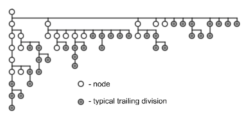
\includegraphics [scale=1.5] {trailing.pdf}
		\caption{A simple schema of the location of \textit{trailing divisions}.}
		\label{fig:trailing}
	\end{figure}
	%	
	Horizontally the above phenomenon can be visualised as the ordered set of all children of any node being statistically similar to the ordered set of all children of the node except the first one. It is a direct effect of the Tree-Structured Stick Breaking process (TSSB)~\cite{ghahramani2010tree}. Similarly to the above, from a vertical point of view, in any tree where $\lambda = 1$ all sub-trees of a node are statistically similar to that node. In the presented experimental data, these trailing divisions are visible as the falling off "tail" in the data per level histograms as well as the cause of the high deviation of width within the tree. Unfortunately, due to the nature of the TSSB distribution, it is impossible to avoid this behaviour without post-processing. No forms of such post-processing were employed for the experiments presented in this paper.
    
    As an additional observation to the above, the $\gamma$ value does not change by level. Because of this, a critical factor in considering how many children a node will have is the number of data passing through the node. Bigger nodes that are located higher up are more likely to have more children than smaller nodes lower down the hierarchy. Additionally, the more children a node has, the more of them will be small nodes, i.e., nodes through which few objects pass, resulting primarily in leaf nodes or nodes with single children. This behaviour of smaller nodes also transfers lower down the hierarchy where less data reaches leading to similar behaviour.
    
    Finally, the reassigned test cases show a tendency for data to move down hierarchy levels. Intuitively the groups located lower down in the hierarchy are more specific and potentially conflicting data would be prone to moving down into the more specific child clusters. However, despite this tendency, the hierarchies retain most of their previous characteristics, simply with the mass of data being shifted down towards the lower levels of the hierarchy. Due to the post-processing applied to these datasets, they can be better su	ited for initial testing of grouping methods. In most cases, testing using both types of datasets (unfiltered and filtered) may be the preferred and most valuable approach in every case where the features of the objects are considered. 
    
	\section{Benchmarking Dataset}
    \label{sec:benchmarking_dataset}
    To establish a benchmarking dataset, representative hierarchies have been chosen from all of the generated ones. For every parameter set-up, from~\Cref{tab:parameter-configurations} (separately for the reassignment procedure and without it) average values of created hierarchies were calculated. The averages cover the statistics reported in the~\Cref{experiments}. After that, the Euclidean distance was calculated between all the generated hierarchies and the corresponding average values so that the top 10 closest datasets were identified. The final collection of 160 hierarchies is publicly available and might be used for benchmarking purposes (\texttt{http://kio.pwr.edu.pl/?page\_id=396}).
	%
	\section{Conclusions}
	\label{conclusion}
	The experiments presented in the previous sections serve to highlight both strengths and weaknesses of the proposed generator. A prominent strength is a high range of different tree structures that can be generated and the ability to fine-control these structures using the introduced parameters. Thanks to that, a wide range of different hierarchy types, often seen in the real-world problems, has been generated and made publicly available\footnote{\url{https://cs.nyu.edu/~roweis/data.html}}. 
	
	Published benchmarks and the ability to create more hierarchies using the generator is lying a solid foundation for further development of the concept of Object Cluster Hierarchies. Generated hierarchies can assist not only in clustering methods development and comparison but also in a research of OCH quality measures. The latter is important since the differences between OCH and Hierarchical Clustering results are not fully recognised by existing internal and external measures. 
	
	From a practical point of view, it is also essential that the generator's parameters can be separated into groups, each controlling a different aspect of the hierarchy. Vertical distribution of data is controlled by $\alpha_0$ and $\lambda$, hierarchy width depends on the value of $\gamma$, and $p$, $q$ controls the data specificity. As shown in this article, every parameter set has an interpretation and its effect on the generated hierarchy is straightforward. This allows for a further fine-tuning towards desired test data. The generation process scales with the number of points to generate, expanding the hierarchy as more elements are generated.
    
    One of the findings is the fact that the generated hierarchy will always display a degree of self-similarity, replicating the same general form both vertically and horizontally. We called it as generation of trailing divisions. Because of that a few specific areas of the generated hierarchies are not fully controlled. A remedy for this issue is to use a post-processing procedure similar to the described reassignment process. This should result in cleaner hierarchies and give the user finer control over their overall structure.
    
    In its current form, the generator is limited to a generation of normally-distributed, multidimensional, and uncorrelated real value data. It can be extended to use different kernels leading to different structures of generated hierarchies or generators operating on different types of data.
    
    Furthermore, the self-similar (fractal) nature of the hierarchies suggests a potential for the generator to be described using the language of fractals and especially L-Systems~\cite{prusinkiewicz2013lindenmayer}. Describing the generation process in that form may provide a different (more granular) view over the details of the hierarchical structure. 
	%
	\bibliography{mybibfile}
	%
\end{document}